%% abtex2-modelo-trabalho-academico.tex, v-1.9.6 laurocesar
%% Copyright 2012-2016 by abnTeX2 group at http://www.abntex.net.br/ 
%%
%% This work may be distributed and/or modified under the
%% conditions of the LaTeX Project Public License, either version 1.3
%% of this license or (at your option) any later version.
%% The latest version of this license is in
%%   http://www.latex-project.org/lppl.txt
%% and version 1.3 or later is part of all distributions of LaTeX
%% version 2005/12/01 or later.
%%
%% This work has the LPPL maintenance status `maintained'.
%% 
%% The Current Maintainer of this work is the abnTeX2 team, led
%% by Lauro César Araujo. Further information are available on 
%% http://www.abntex.net.br/
%%https://preview.overleaf.com/public/ddhdfzwmzvkc/images/f044e18a052fdcacf45438282ae6b4d3dcdd0802.jpeg
%% This work consists of the files abntex2-modelo-trabalho-academico.tex,
%% abntex2-modelo-include-comandos and abntex2-modelo-references.bib
%%

% ------------------------------------------------------------------------
% ------------------------------------------------------------------------
% abnTeX2: Modelo de Trabalho Academico (tese de doutorado, dissertacao de
% mestrado e trabalhos monograficos em geral) em conformidade com 
% ABNT NBR 14724:2011: Informacao e documentacao - Trabalhos academicos -
% Apresentacao
% ------------------------------------------------------------------------
% ------------------------------------------------------------------------

\documentclass[
	% -- opções da classe memoir --
	12pt,				% tamanho da fonte
	openright,			% capítulos começam em pág ímpar (insere página vazia caso preciso)
	oneside,			% para impressão em recto e verso. Oposto a oneside
	a4paper,			% tamanho do papel. 
	% -- opções da classe abntex2 --
	%chapter=TITLE,		% títulos de capítulos convertidos em letras maiúsculas
	%section=TITLE,		% títulos de seções convertidos em letras maiúsculas
	%subsection=TITLE,	% títulos de subseções convertidos em letras maiúsculas
	%subsubsection=TITLE,% títulos de subsubseções convertidos em letras maiúsculas
	% -- opções do pacote babel --
	english,			% idioma adicional para hifenização
	french,				% idioma adicional para hifenização
	spanish,			% idioma adicional para hifenização
	brazil				% o último idioma é o principal do documento
	]{abntex2}

% ---
% Pacotes básicos 
% ---
\usepackage{lmodern}			% Usa a fonte Latin Modern			
\usepackage[T1]{fontenc}		% Selecao de codigos de fonte.
\usepackage[utf8]{inputenc}		% Codificacao do documento (conversão automática dos acentos)
\usepackage{lastpage}			% Usado pela Ficha catalográfica
\usepackage{indentfirst}		% Indenta o primeiro parágrafo de cada seção.
\usepackage{color}				% Controle das cores
\usepackage{graphicx}			% Inclusão de gráficos
\usepackage{microtype} 	% para melhorias de justificação
\usepackage{caption}
\usepackage{listings}
\lstset{
numbers=left, 
numberstyle=\small, 
numbersep=8pt, 
frame = single,
breaklines=true,
language=Python, 
framexleftmargin=15pt}
% ---
		
% ---
% Pacotes adicionais, usados apenas no âmbito do Modelo Canônico do abnteX2
% ---
\usepackage[combrasao]{abntex2-pucminas}
\usepackage{acronym}
% ---

% ---
% Pacotes de citações
% ---
%\usepackage[brazilian,hyperpageref]{backref}	 % Paginas com as citações na bibl
%\usepackage[alf]{abntex2cite}	% Citações padrão ABNT

% ---
% Informações de dados para CAPA e FOLHA DE ROSTO
% ---
% Coloque o título em caixa alta. É o padrão da PUC.
\titulo{Arquitetura de Data Lake para Análise de Dados do Legislativo brasileiro}
\autor{Giorge Caique Pinheiro de Souza Luiz}
\local{Belo Horizonte}
\data{2020}
\orientador{Prof. Sandro Jerônimo de Almeida}
%\coorientador{Professor}
\instituicao{%
    Pontifícia Universidade Católica de Minas Gerais
}
\departamento{%
     Curso de Bacharelado em Sistemas de Informação
}
\tipotrabalho{Monografia}
% O preambulo deve conter o tipo do trabalho, o objetivo, 
% o nome da instituição e a área de concentração 
\preambulo{}
% ---


% ---
% Configurações de aparência do PDF final

% alterando o aspecto da cor azul
\definecolor{blue}{RGB}{41,5,195}

% informações do PDF
\makeatletter
\hypersetup{
     	%pagebackref=true,
		pdftitle={\@title}, 
		pdfauthor={\@author},
    	pdfsubject={\imprimirpreambulo},
	    pdfcreator={LaTeX with abnTeX2},
		pdfkeywords={abnt}{latex}{abntex}{abntex2}{trabalho acadêmico}, 
		colorlinks=true,       		% false: boxed links; true: colored links
    	linkcolor=blue,          	% color of internal links
    	citecolor=blue,        		% color of links to bibliography
    	filecolor=magenta,      		% color of file links
		urlcolor=blue,
		bookmarksdepth=4
}
\makeatother
% --- 

% --- 
% Espaçamentos entre linhas e parágrafos 
% --- 

% O tamanho do parágrafo é dado por:
\setlength{\parindent}{1.3cm}

% Controle do espaçamento entre um parágrafo e outro:
\setlength{\parskip}{0.2cm}  % tente também \onelineskip

% ---
% compila o indice
% ---
\makeindex
% ---

% ----
% Início do documento
% ----
\begin{document}

% Seleciona o idioma do documento (conforme pacotes do babel)
%\selectlanguage{english}
\selectlanguage{brazil}

% Retira espaço extra obsoleto entre as frases.
\frenchspacing 

% ----------------------------------------------------------
% ELEMENTOS PRÉ-TEXTUAIS
% ----------------------------------------------------------
% \pretextual

% ---
% Capa
% ---
\imprimircapa
% ---

% ---
% Folha de rosto
% (o * indica que haverá a ficha bibliográfica)
% ---
\imprimirfolhaderosto*
% ---

% ---
% Inserir a ficha bibliografica
%% ---
% Inserir a ficha bibliografica
% ---
% Ficha catalográfica
% INCLUIR O ARQUIVO PDF GERADO PELA BIBLIOTECA COMO FIGURA.
\begin{fichacatalografica}
    \includepdf{fig_ficha_catalografica.pdf}
\end{fichacatalografica}

% Isto é um exemplo de Ficha Catalográfica, ou ``Dados internacionais de
% catalogação-na-publicação''. Você pode utilizar este modelo como referência. 
% Porém, provavelmente a biblioteca da sua universidade lhe fornecerá um PDF
% com a ficha catalográfica definitiva após a defesa do trabalho. Quando estiver
% com o documento, salve-o como PDF no diretório do seu projeto e substitua todo
% o conteúdo de implementação deste arquivo pelo comando abaixo:
%
% \begin{fichacatalografica}
%     \includepdf{fig_ficha_catalografica.pdf}
% \end{fichacatalografica}

%\begin{fichacatalografica}
%	\sffamily
%	\vspace*{\fill}					% Posição vertical
%	\begin{center}					% Minipage Centralizado
%	\fbox{\begin{minipage}[c][8cm]{13.5cm}		% Largura
%	\small
%	\imprimirautor
%	%Sobrenome, Nome do autor
%	
%	\hspace{0.5cm} \imprimirtitulo  / \imprimirautor. --
%	\imprimirlocal, \imprimirdata-
%	
%	\hspace{0.5cm} \pageref{LastPage} p. : il. (algumas color.) ; 30 cm.\\
%	
%	\hspace{0.5cm} \imprimirorientadorRotulo~\imprimirorientador\\
%	
%	\hspace{0.5cm}
%	\parbox[t]{\textwidth}{\imprimirtipotrabalho~--~\imprimirinstituicao,
%	\imprimirdata.}\\
%	
%	\hspace{0.5cm}
%		1. Palavra-chave1.
%		2. Palavra-chave2.
%		2. Palavra-chave3.
%		I. Orientador.
%		II. Universidade xxx.
%		III. Faculdade de xxx.
%		IV. Título 			
%	\end{minipage}}
%	\end{center}
%\end{fichacatalografica}
% ---

% ---

% ---
% Inserir errata
%% ---
% Inserir errata
% ---
\begin{errata}
Elemento opcional da \citeonline[4.2.1.2]{NBR14724:2011}. Exemplo:

\vspace{\onelineskip}

FERRIGNO, C. R. A. \textbf{Tratamento de neoplasias ósseas apendiculares com
reimplantação de enxerto ósseo autólogo autoclavado associado ao plasma
rico em plaquetas}: estudo crítico na cirurgia de preservação de membro em
cães. 2011. 128 f. Tese (Livre-Docência) - Faculdade de Medicina Veterinária e
Zootecnia, Universidade de São Paulo, São Paulo, 2011.

\begin{table}[htb]
\center
\footnotesize
\begin{tabular}{|p{1.4cm}|p{1cm}|p{3cm}|p{3cm}|}
  \hline
   \textbf{Folha} & \textbf{Linha}  & \textbf{Onde se lê}  & \textbf{Leia-se}  \\
    \hline
    1 & 10 & auto-conclavo & autoconclavo\\
   \hline
\end{tabular}
\end{table}

\end{errata}
% ---

% ---

% ---
% Inserir folha de aprovação
%% ---
% Inserir folha de aprovação
% ---

% Isto é um exemplo de Folha de aprovação, elemento obrigatório da NBR
% 14724/2011 (seção 4.2.1.3). Você pode utilizar este modelo até a aprovação
% do trabalho. Após isso, substitua todo o conteúdo deste arquivo por uma
% imagem da página assinada pela banca com o comando abaixo:
%
% \includepdf{folhadeaprovacao_final.pdf}
%
\begin{folhadeaprovacao}
    
    \begin{center}
        {\ABNTEXchapterfont\large\imprimirautor}
        
        \vspace*{\fill}\vspace*{\fill}
        \begin{center}
            \ABNTEXchapterfont\bfseries\Large\imprimirtitulo
        \end{center}
        \vspace*{\fill}
        
        \hspace{.45\textwidth}
        \begin{minipage}{.5\textwidth}
            \imprimirpreambulo
        \end{minipage}%
        \vspace*{\fill}
    \end{center}
    
    Trabalho aprovado. \imprimirlocal, 25 de dezembro de 2016:
    
    \assinatura{\textbf{\imprimirorientador} \\ PUC Minas (Orientador)} 
    \assinatura{\textbf{Professor} \\ UFEXTERNA (Banca Examinadora)}
    \assinatura{\textbf{Professor} \\  PUC Minas (Banca Examinadora)}
    %\assinatura{\textbf{Professor} \\ Convidado 3}
    %\assinatura{\textbf{Professor} \\ Convidado 4}
    
    \begin{center}
        \vspace*{0.5cm}
        {\large\imprimirlocal}
        \par
        {\large\imprimirdata}
        \vspace*{1cm}
    \end{center}
    
\end{folhadeaprovacao}
% ---

%versao antiga
%% Termo de Aprovação
%
%% Texto da aprovação
%\textoaprovacao{Dissertação apresentada ao Programa de Pós-Graduação em Informática da Pontifícia Universidade Católica de Minas Gerais,
%como requisito parcial para obtenção do título de Mestre em Informática.}
%%\onehalfspacing
%%\onehalfspacing
%%\onehalfspacing
%% Primeira assinatura
%\primeiroassina{Prof. Dr. Orientador -- PUC Minas (Orientador)}
%
%% Segunda assinatura
%\segundoassina{Prof. Dr. Membro Externo -- UFEXTERNA (Banca Examinadora)}
%%$^{a}$
%% Terceira assinatura
%\terceiroassina{Prof. Dr. Membro Interno -- PUC Minas (Banca Examinadora)}
%
%% Quarta assinatura
%%\quartoassina{}
%
%% Data da defesa
%\localdia{Belo Horizonte, 06 de julho de 2015.}
%
%% Gera o termo de aprovação
%\termodeaprovacao
% ---


% ---
% Dedicatória
%% Dedicatória
\begin{dedicatoria}
    \vspace*{\fill}
    \centering
    \noindent
    \textit{ Este trabalho é dedicado às crianças adultas que,\\
        quando pequenas, sonharam em se tornar cientistas.} \vspace*{\fill}
\end{dedicatoria}
% ---

% ---

% ---
% Agradecimentos
%\begin{agradecimentos}
    Os agradecimentos principais são direcionados à Gerald Weber, Miguel Frasson,
    Leslie H. Watter, Bruno Parente Lima, Flávio de Vasconcellos Corrêa, Otavio Real
    Salvador, Renato Machnievscz\footnote{Os nomes dos integrantes do primeiro
        projeto abn\TeX\ foram extraídos de
        \url{http://codigolivre.org.br/projects/abntex/}} e todos aqueles que
    contribuíram para que a produção de trabalhos acadêmicos conforme
    as normas ABNT com \LaTeX\ fosse possível.
    
    Agradecimentos especiais são direcionados ao Centro de Pesquisa em Arquitetura
    da Informação\footnote{\url{http://www.cpai.unb.br/}} da Universidade de
    Brasília (CPAI), ao grupo de usuários
    \emph{latex-br}\footnote{\url{http://groups.google.com/group/latex-br}} e aos
    novos voluntários do grupo
    \emph{\abnTeX}\footnote{\url{http://groups.google.com/group/abntex2} e
        \url{http://www.abntex.net.br/}}~que contribuíram e que ainda
    contribuirão para a evolução do \abnTeX.
    
\end{agradecimentos}
% ---

% ---

% ---
% Epígrafe
%% Epígrafe
\begin{epigrafe}
    \vspace*{\fill}
    \begin{flushright}
        \textit{``Não vos amoldeis às estruturas deste mundo, \\
            mas transformai-vos pela renovação da mente, \\
            a fim de distinguir qual é a vontade de Deus: \\
            o que é bom, o que Lhe é agradável, o que é perfeito.\\
            (Bíblia Sagrada, Romanos 12, 2)}
    \end{flushright}
\end{epigrafe}
% ---

% ---

% ---
% RESUMOS
% resumo em português
% Resumo em portugues
\setlength{\absparsep}{18pt} % ajusta o espaçamento dos parágrafos do resumo
\begin{resumo}
        Este estudo aborda a modelagem e implementação de uma plataforma que possibilite a análise de dados referentes a Câmara dos Deputados do Brasil, a qual faz parte do Poder Legislativo da União. Utilizou-se de técnicas de Big Data e Cloud Computing com o intuito de propor o estado da arte para uma arquitetura de análise de dados políticos. Foram utilizadas como fontes de dados os dados abertos disponibilizados pela Câmara dos Deputados, o monitoramento das atividades dos parlamentares nas redes sociais, e as notícias que referenciem os políticos do Legislativo. A partir desta base, análises descritivas sobre as atividades parlamentares foram realizadas, além de estudos que identificam as correlações entre os discursos políticos dos deputados na mídia e o que é efetivamente realizado na Câmara.
        
    
    \textbf{Palavras-chave}: Big Data, Câmara dos Deputados, Twitter, Data Lake, Cloud Computing.
\end{resumo}


% resumo em inglês
%\begin{resumo}[Abstract]
    \begin{otherlanguage*}{english}
        This is the english abstract.
        
        \vspace{\onelineskip}
        
        \noindent 
        \textbf{Keywords}: latex. abntex. text editoration.
    \end{otherlanguage*}
\end{resumo}

% resumo em francês 
%\begin{resumo}[Résumé]
 \begin{otherlanguage*}{french}
    Il s'agit d'un résumé en français.
 
   \textbf{Mots-clés}: latex. abntex. publication de textes.
 \end{otherlanguage*}
\end{resumo}

% resumo em espanhol
%% resumo em espanhol
\begin{resumo}[Resumen]
 \begin{otherlanguage*}{spanish}
   Este es el resumen en español.
  
   \textbf{Palabras clave}: latex. abntex. publicación de textos.
 \end{otherlanguage*}
\end{resumo}
% ---

% ---


% ---
% inserir lista de ilustrações
% ---
%\pdfbookmark[0]{\listfigurename}{lof}
\listoffigures*
%\cleardoublepage
% ---


% ---
% inserir lista de gráficos
% ---
%\pdfbookmark[0]{\listgraficoname}{lop}
%{
%    \makeatletter
%    \renewcommand\numberline[1]{
%        \leftskip 0em
%        \rightskip 1.6em
%        \parfillskip -\rightskip
%        \parindent 0em
%        \@tempdima 2.0em
%        \vspace{0.5em} \advance\leftskip \@tempdima \null\nobreak\hskip -\leftskip
%        GRÁFICO \normalfont #1 -- }
%    \makeatother
%    
%    \listofgraficos
%}
%\cleardoublepage
% ---


% ---
% inserir lista de tabelas
% ---
\pdfbookmark[0]{\listtablename}{lot}
%\listoftables*
%\cleardoublepage
% ---

% ---
% inserir lista de quadros
% ---
\pdfbookmark[0]{\listquadroname}{loq}
{
\makeatletter
\renewcommand\numberline[1]{
    \leftskip 0em
    \rightskip 1.6em
    \parfillskip -\rightskip
    \parindent 0em
    \@tempdima 2.0em
    \vspace{0.5em} \advance\leftskip \@tempdima \null\nobreak\hskip -\leftskip
    QUADRO \normalfont #1 -- }
\makeatother

%\listofquadros
}
%\cleardoublepage
% ---




% ---
% inserir lista de abreviaturas e siglas
% Lista de Abreviaturas e Siglas
\begin{abreviaturas}
    \acro{DW}{\textit{Data Warehouse}}
    \acro{ETL}{\textit{Extract, Transform and Load}}
    \acro{ELT}{\textit{Extract, Load and Transform}}
    \acro{IA}{Inteligência Artificial}
    \acro{API}{\textit{Application Programming Interface}
    \acro{EDA}{\textit{Exploratory data analysis}}
\end{abreviaturas}

% ---

% ---
% inserir lista de símbolos
%\begin{simbolos}
  \item[$ \Gamma $] Letra grega Gama
  \item[$ \Lambda $] Lambda
  \item[$ \zeta $] Letra grega minúscula zeta
  \item[$ \in $] Pertence
\end{simbolos}

% ---
% ---

% ---
% inserir o sumario
% ---
\pdfbookmark[0]{\contentsname}{toc}
\tableofcontents*
%\cleardoublepage
% ---



% ----------------------------------------------------------
% ELEMENTOS TEXTUAIS
% ----------------------------------------------------------
\textual

% ----------------------------------------------------------
% PARTE
% ----------------------------------------------------------
%\part{Referenciais teóricos}
% ----------------------------------------------------------


% ----------------------------------------------------------
% CAPÍTULOS
% ----------------------------------------------------------



\chapter{Introdução}
% Label para referenciar
\label{introducao}
% Texto do capítulo

\section{Problema}
A verdade pode ser definida de duas formas. A verdade racional, definida a partir de um embasamento científico, e a verdade factual, esta, por sua vez, se apoiando nas relações humanas. Esta segunda possui maior importância no âmbito político, uma vez que a verdade racional é, a não ser que se prove através dos mesmos critérios aplicadas pelo método científico, irrefutável. Logo, ao prover a ambiguidade da verdade, se torna um importante artifício para a articulação de atos políticos \cite{entrepassadofuturo}.

É sabido que com os avanços da tecnologia, os regimes democráticos ao redor do globo vêm sofrendo com a desinformação da população. Observa-se, por exemplo, a influência que as \textit{fake news} e os \textit{bots} possuem nos processos eleitorais das sociedades democráticas contemporâneas \cite{fakenewsbot}.

Ao final da campanha presidencial americana de 2016, podê-se observar que as 20 notícias falsas com maior engajamento na internet possuíam mais compartilhamentos, \textit{likes} e comentários do que as 20 reportagens produzidas pela mídia tradicional com melhor desempenho no Facebook \cite{facebookamericananalysis}. 

Em seus primeiros doze meses de governo, o atual presidente da república do Brasil, Jair Messias Bolsonaro, deferiu 608 declarações falsas ou distorcidas em discursos, entrevistas e mídias sociais. Do total de declarações do presidente, 56\% delas possuem algum grau de distorção \cite{declaracoesbolsonaro}.

Em contrapartida, observa-se também uma discussão sobre como a tecnologia pode prestar um papel crucial nos processos decisórios em uma Democracia Digital. Como novos modelos de tomadas de decisão do Estado podem ser adaptados com o intuito de promover uma maior participação e engajamento da esfera civil \cite{democraciadigital}.

Um cenário onde a população está participando ativamente das atividades políticas, mas que também sofre com as estratégias que promovem a desinformação como artifício político. Considerando essa nova realidade, presume-se que informar a população através de fontes oficiais torna-se uma alternativa coerente.

\section{Objetivo Geral}
O objetivo deste trabalho consiste na criação de um repositório unificado contendo informações tratadas, verificadas e referenciadas que contemplem uma visão geral das atividades exercidas no Legislativo brasileiro, especificamente, a Câmara dos Deputados. A partir deste repositório, foram realizadas análises exploratórias que descrevem informações relacionadas às atividades parlamentares, especificamente analisando os gastos reembolsando as despesas dos deputados, as proposições submetidas à Câmara, temas dessas proposições, conteúdo dos \textit{tweets} dos perfis oficiais dos parlamentares além das notícias que os citam. Análises mais criteriosas relacionando o conteúdo das proposições com as notícias dos deputados e suas atividades no Twitter foram aplicadas com uma amostra dos deputados.

\section{Objetivos Específicos}
Visando atingir o objetivo geral, os objetivos específicos são:
\begin{enumerate} 
 \item [a)] Mapear as fontes de dados que serão utilizadas; 
 \item [b)] Elencar as tecnologias necessárias para o desenvolvimento;
 \item [c)] Projetar a arquitetura deste projeto;
 \item [d)] Implementar o projeto;
 \item [e)] Gerar indicadores gerais das atividades dos parlamentares;
 \item [f)] Elencar deputados para análises mais criteriosas.
\end{enumerate} 

\chapter{Revisão Bibliográfica}
% Label para referenciar
\label{revisao}
Neste capítulo, os conceitos fulcrais para o entendimento e desenvolvimento do projeto são abordados e detalhados.

\section{Democracia} Pode-se observar a existência de dois tipos principais de democracia ao redor do globo. A Democracia Direta, também conhecida como Democracia Pura, na qual todos os cidadãos detêm o poder de participar diretamente do processo de tomada de decisão. Os modelos atuais de democracia seguem a vertente da Democracia Representativa, na qual indivíduos são eleitos para representar os interesses de determinado grupo no processo de tomada de decisão do Estado \cite{impactofictonreiforcingcitizens}. 

Alguns autores defendem que a Democracia Direta seria mais adequada em uma sociedade democrática considerando a efetividade de sua participação nos processos decisórios, porém este modelo apresenta uma impossibilidade técnica de ser utilizada, fator esse que pode ser reavaliado conforme a tecnologia vem tornando-se cada vez mais presente em nossa sociedade \cite{impactofictonreiforcingcitizens}.

\section{\textit{Cloud Computing}} \textit{Cloud Computing} ou Computação em Nuvem define uma modalidade de computação que se diferencia pela disponibilização de recursos computacionais, sendo esses recursos infraestrutura, plataforma, \textit{software}, serviços ou armazenamento, de maneira dinâmica e escalável sob demanda \cite{cloudcomputing}. 

Trata-se de um ambiente compartilhado entre vários usuários onde o custo desses recursos segue a lógica de \textit{pay as you go}, ou seja, o usuário é cobrado pelo tempo de utilização de determinado recurso na plataforma de \textit{Cloud}. O fator crucial que permitiu aos provedores de \textit{Cloud} o gerenciamento e segurança desse ambiente é a virtualização, uma vez que torna-se possível o isolamento de aplicações sendo executadas no mesmo \textit{hardware}\cite{cloudcomputing}.

\section{\textit{Big Data}} O termo \textit{Big Data} teve sua primeira aparição como uma tecnologia emergente em 2011 pelo Gartner, em sua análise denominada \textit{Hype Cycle for Emerging Technologies}, que identifica novas tendências no cenário tecnológico mundial, além de reconhecer o ponto em que se encontra \cite{bigdataincontext}.

O \textit{Hype Cycle} do Gartner foi introduzido em 1995 com o intuito de descrever o progresso das tecnologias emergentes no mercado através de uma curva, denominada como \textit{Hype Curve} \cite{understandinghypecicles}.

% Figura
\begin{figure}[!ht]
	\centering	
	\caption[\hspace{0.1cm}Fases do \textit{Hype Cycle}]{Fases do \textit{Hype Cycle}}
	  \vspace{-0.4cm}
	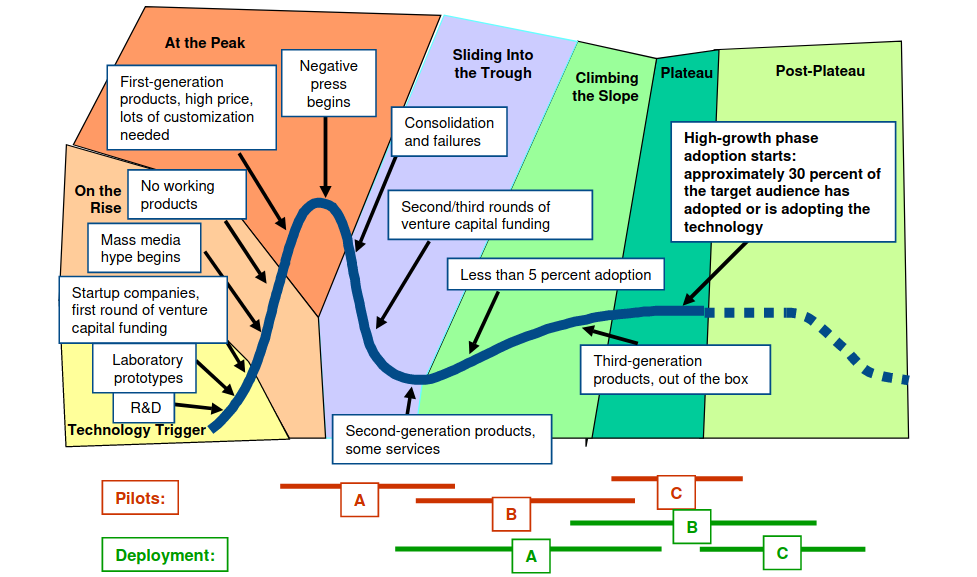
\includegraphics[width=.8\textwidth]{TCC/figuras/explaining_hype_cycle.png}
	% Caption centralizada
% 	\captionsetup{justification=centering}
	% Caption e fonte
	 \vspace{-0.3cm}
	\\\textbf{\footnotesize Fonte: Gartner Research}
	\label{fig:tela1}
\end{figure}

Esse ciclo segue as seguintes fases:

\begin{itemize}
\item \textbf{\textit{Technology Trigger}}: Demonstração de protótipos e pesquisas em laboratório que provocam interesse do público e da indústria;
\item \textbf{\textit{On the Rise}}: Caracterizada pelas expectativas infladas, essa fase é marcada pelo impacto potencial que essa tecnologia terá no mercado e na sociedade como um todo. Primeiras gerações de produtos que demonstram pouca usabilidade, alta especificidade e custos altos de produção/implementação;
\item \textbf{\textit{At the Peak of Inflated Expectations}}: Após a disponibilização da primeira geração dos produtos, a tecnologia é levada aos seus limites conforme a distribuição e o uso são ampliados. As empresas começam a analisar a viabilidade e o benefício de aderir a tecnologia;
\item \textbf{\textit{Sliding Into the Trough of Disillusionment}}: O vale da desilusão ocorre quando a tecnologia falha ao buscar atender as expectativas infladas criadas pela mídia e é desacreditada. Nessa etapa, os produtos são melhorados com os \textit{feedbacks} dos clientes e tenta-se destacar os benefícios de adotar essa tecnologia;
\item \textbf{\textit{Climbing the Slope of Enlightenment}}: Experiências reais e experimentações aumentam em diversos segmentos, levando à um melhor entendimento da tecnologia. Novas gerações de produtos são desenvolvidas e empresas mais flexíveis e tecnologicamente agressivas passam à adotá-la;
\item \textbf{\textit{Entering the Plateau of Productivity}}: Essa fase significa a entrada da tecnologia para a adoção do público \textit{mainstream}, onde os benefícios da tecnologia já são publicamente reconhecidos. Usualmente essas tecnologias são absorvidas em ecossistemas tecnológicos que ampliam sua adoção e sua maturidade; 
\item \textbf{\textit{Post-Plateau}}: Nesta fase a tecnologia já passou por todas as etapas e já se consolidou como parte do cenário tecnológico.
\end{itemize}


% Figura
\begin{figure}[!ht]
	\centering	
	\caption[\hspace{0.1cm}\textit{Big Data} no \textit{Hype Cycle}]{\textit{Big Data} no \textit{Hype Cycle}}
	  \vspace{-0.4cm}
	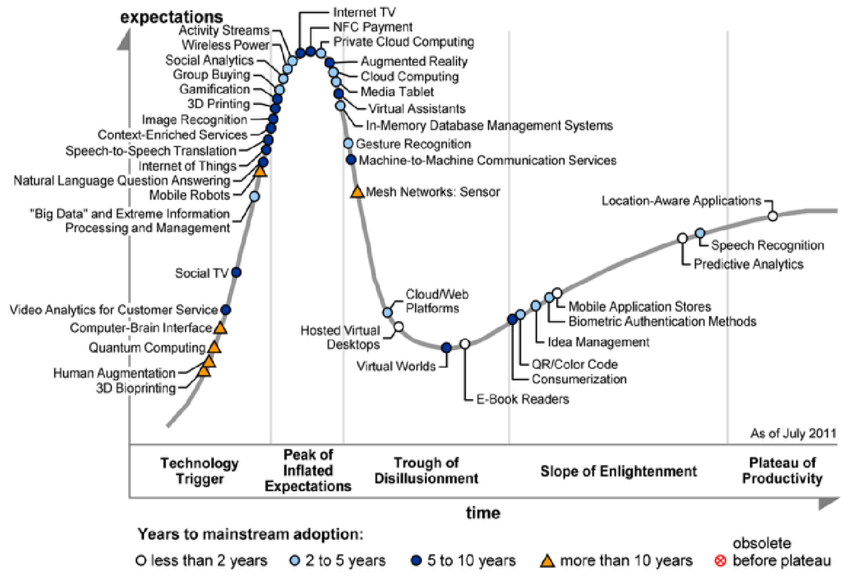
\includegraphics[width=.8\textwidth]{TCC/figuras/Hype-Cycle-for-emerging-technologies-Source-Gartner-Group-2011.png}
	% Caption centralizada
% 	\captionsetup{justification=centering}
	% Caption e fonte
	 \vspace{-0.3cm}
	\\\textbf{\footnotesize Fonte: Gartner}
	\label{fig:tela1}
\end{figure}

\textit{Big Data} pode ser definido como um cenário onde existe uma volumetria massiva de dados com expressiva heterogeneidade de tal forma que se torna inviável utilizando os métodos e tecnologias tradicionais. Dados estruturados, semi-estruturados e não estruturados precisam ser extraídos e analisados, porém essa complexidade torna impossível o gerenciamento e processamento nos moldes tradicionais. Para este ambiente, temos 3 pontos basilares deste conceito emergente, também comumente conhecidos como os 3 V's de Big Data \cite{bigdatafastdatadatalake}. São eles:
\begin{itemize} 
 \item \textbf{Volume}: Trata-se de uma volumetria absurda de dados; 
 \item \textbf{Variedade}: Dados caracterizados por sua heterogeneidade, sendo eles estruturados, semi-estruturados e não estruturados;
 \item \textbf{Velocidade}: Altíssima velocidade em que os dados são gerados e processados.
\end{itemize}

\section{\textit{Extract, Transform and Load (ETL)}} Um sistema ou processo de \ac{ETL} pode ser considerado como tudo entre a origem do dado e a camada de apresentação do seu sistema analítico. Consiste em três etapas principais:
\begin{itemize}
\item \textbf{\textit{Extract}}: A extração é o primeiro passo de um processo de ETL. É a etapa onde os dados necessários para análise precisam ser extraídos dos sistemas de origem e inseridos no ambiente analítico para as manipulações necessárias;
\item \textbf{\textit{Transform}}: Uma vez que o dado já está no ambiente analítico e pode ser facilmente analisado, inicia-se a etapa de transformação, que consiste em corrigir e normalizar o dado (tipagem, valores nulos, conflitos de domínio), além de relacionar múltiplas fontes de dados para agregar o valor máximo para o negócio;
\item \textbf{\textit{Load}}: A última etapa do processo é caracterizada pela carga ou inserção dos dados processados na etapa de transformação em um ambiente analítico.
\end{itemize}
Ao final deste processo , as bases de dados estarão atualizados e os dados serão disponibilizados para ferramentas de análise e visualização que proverão os resultados para as partes interessadas \cite{thedatawarehousetoolkit}.

\section{\textit{Data Lake}} Se tratando do conceito de \textit{Data Lake}, sua estrutura é mais flexível. O \textit{Data Lake} pode ser definido como um repositório massivo, centralizado e escalável de dados, contendo dados em seu formato de origem, além de possibilitar sua ingestão e processamento neste ambiente \cite{bigdatafastdatadatalake}. 

Uma pecualiaridade do \textit{Data Lake} é a separação do processamento e do armazenamento. Quando comparado  com o \textit{Data Warehouse}, por exemplo, um servidor ou mesmo um cluster de servidores possuem a unidade de processamento e de armazenamento nos mesmos nós. Ou seja, uma instância e responsável pela execução das consultas aplicadas à ele e também do armazenamento dos dados propriamente ditos. Com a ascenção das tecnologias de \textit{Cloud Computing}, temos o barateamento dos serviçõs de \textit{storage}, fator essencial para a construção de um \textit{Data Lake}, onde temos um \textit{storage} escalável e o processamento é realizado à parte, onde utiliza-se de computação distribuída sob demanda \cite{datalakeforenterprises}. 

Geralmente, o \textit{Data Lake} é segmentado em zonas, baseado nas condições e nos objetivos que os dados que cada zona possui. Algumas das zonas são:

\begin{itemize}
 \item \textbf{\textit{Raw Zone}}: A \textit{Raw Zone} é a zona onde os dados são importados. Nesta zona, os dados não sofrem alteração alguma e o seu formato é exatamente igual ao disponibilizado pelo sistema de origem; 
 \item \textbf{\textit{Staged Zone}}: Na \textit{Staged Zone}, os dados já sofrem transformações com o intuito de padronizar os dados. Transformações como de/paras, transformação de \textit{encoding}, formatos de data, entre outras. Operações que tem o único objetivo de manter todos os dados na mesma estrutura para análises posteriores;
 \item \textbf{\textit{Curated Zone}}: Na \textit{Curated Zone}, os dados já estão completamente tratados e prontos para as análises dos usuários de negócio. Inclusive teremos resultados de análises que serão disponibilizados aos usuários e \textit{stackholders}.
 \end{itemize}
 
 Essa separação em zonas possibilita uma flexibilidade na exploração de dados que possibilita aos Cientistas de Dados aplicarem seus modelos de \textit{Machine Learning} nas zonas onde a granularidade dos dados é menor, por exemplo a \textit{Staged Zone}, enquanto os indicadores de negócio podem ser gerados a partir dos dados curados e prontos para análise na \textit{Curated Zone} \cite{datalakeforenterprises}.

\section{Spark} O Apache Spark pode ser definido como uma \textit{engine} computacional de alta velocidade e de propósito geral utilizada para o processamento distribuído de grandes massas de dados. Contém módulos com objetivos específicos, sendo eles \cite{learningspark}:

% Figura
\begin{figure}[!ht]
	\centering	
	\caption[\hspace{0.1cm} Spark]{Arquitetura Spark}
	  \vspace{-0.4cm}
	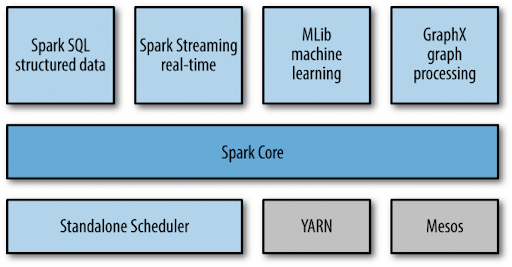
\includegraphics[width=.8\textwidth]{TCC/figuras/spark.png}
	% Caption centralizada
% 	\captionsetup{justification=centering}
	% Caption e fonte
	 \vspace{-0.3cm}
	\\\textbf{\footnotesize Fonte: Apache}
	\label{fig:tela1}
\end{figure}

\begin{itemize}
 \item \textbf{\textit{Spark Core}}: Spark Core contém toda a estrutura para o funcionamento do Spark. Os componentes para armazenamento, gerenciamento de memória, agendamento de tarefas, aém de definir as o conceito dos \textit{Resilient Distributed Datasets} (RDDs), o conceito basilar da plataforma; 
 \item \textbf{\textit{Spark SQL structured data}}: Spark SQL é o pacote utilizado para prover a manipulação de dados estruturados. Trabalha com diversas fontes de dados incluindo JSON, CSV, SQL, Parquet, entre outras. Possibilita ao usuário utilizar uma sintaxe SQL para manipulação dos dados, além do conceito dos \textit{Dataframes}, que podem ser definidos como um RDD com um schema e funcionalidades similares ao SQL;
 \item \textbf{\textit{Spark Streaming real-time}}: Spark Streaming é o módulo do Apache Spark capaz de processar dados em \textit{streaming}. Ele é capaz de realizar esse processamento através de micro processos em \textit{batch};
 \item \textbf{\textit{MLib machine learning}}: Pacote que fornece diversas APIs aos usuários para trabalhar com métodos estatísticos e algoritmos de \textit{Machine Learning}. Possui funções prontas de algoritmos de classificação, regressão, clusterização, entre outros. Estes métodos se beneficiam da computação distribuída do Spark Core para realizar o processamento;
 \item \textbf{\textit{GraphX graph processing}}: APIs para manipulação de grafos, além de possibilitar a computação distribuídas dessas estruturas de dados, uma vez que utilizam a implementação do Spark Core.
 \end{itemize}
 
O Spark possui recursos para gerenciar de maneira eficiente e escalabidade dos seus processos, distribuindo o processamento de um único nó à milhares de nós. O componente responsável por esse gerenciamento é o \textit{cluster manager}. O Apache Spark suporta três opções de \textit{managers}, sendo eles o Hadoop YARN, o Apache Mesos e o \textit{cluster manager} disponibilizado dentro do próprio Spark denominado Standalone Scheduler \cite{learningspark}.
 
\subsection{\textit{Resilient Distributed Datasets (RDDs)}}
Uma das abstrações basilares dessa plataforma é o conceito dos \textit{Resilient Distributed Datasets} (RDDs), que por sua vez podem ser definidos como coleções imutáveis e distribuídas de objetos. São separados em partições que possibilitam o processamento distribuído através do \textit{cluster}. Os RDDs possuem dois tipos de operações, sendo eles as \textit{transformations} e as \textit{actions}. Suas operações são baseadas em um conceito da computação denominado \textit{Lazy Evaluation}, que significa que as \textit{transformations}, operações que transformam o dado como métodos \textit{map} ou \textit{filter}, não serão executadas no momento em que são invocadas, mas sim empilhadas e organizadas em uma pilha de instruções que serão aplicadas aos dados quando uma \textit{action}, operação de saída, como uma escrita no \textit{shell} ou em um arquivo, for disparada \cite{learningspark}.

Para este trabalho, o processamento foi realizado principalmente utilizando o Apache Spark, logo, a explicação do seu funcionamento se torna pertinente. 

\section{Trabalhos Relacionados}
\label{Trabalhos Relacionados}
Nos últimos anos, houveram inúmeros projetos que tratam e analisam dados
públicos com o intuito de informar a população brasileira, partindo tanto da esfera pública como da própria sociedade. 

Um dos projetos que trouxe grande engajamento por parte da comunidade para a análise de dados políticos foi o projeto Serenata de Amor que, através do uso de \textit{Machine Learning}, analisa os reembolsos realizados pela Câmara dos Deputados e divulgados em sua plataforma de Dados Abertos, identificando atividades incomuns que possam ser caracterizadas como fraude\footnote{Disponível em <https://serenata.ai/> Acesso em: 19 mai, 2020}. 

O Ministério Público de Minas Gerais publicou o Mapa Social. Uma plataforma sumariza os indicadores sociais de diversas instituições públicas afim de informar a população sobre os diversos indicadores do Estado se tratando das temáticas Educação, Segurança e Saúde\footnote{Disponível em <https://mapasocial.mpmg.mp.br/> Acesso em: 19 mai, 2020}. 

O CELUPPI Advogados é um escritório de advocacia brasileiro e criador do Radar Governamental, projeto focado no monitoramento das atividades do Legislativo, utilizando os Dados Abertos da Câmara dos Deputados para realizar parte das suas atividades de monitoramento\footnote{Disponível em <https://radargovernamental.com.br/sobre/> Acesso em: 19 mai, 2020}.

\chapter{Metodologia}
% Label para referenciar
\label{metodologia}
O estudo apresenta a modelagem e implementação de uma arquitetura que possibilite a extração, processamento e disponibilização dos dados referente à Câmara dos Deputados. Este projeto foi desenvolvido utilizando o Databricks, que pode ser definida como uma plataforma unificada para análise de dados na \textit{Cloud} para um volume massivo de dados, promovendo a colaboração entre Cientistas e Engenheiros de Dados\footnote{Disponível em <https://databricks.com/product/unified-data-analytics-platform> Acesso em: 19 mai, 2020}.
A arquitetura pode ser definida em 3 camadas (serão detalhadas nas seções a seguir):
\begin{enumerate} 
 \item [1)] Armazenamento;
 \item [2)] \textit{Extract, Transform and Load (ETL)};
 \item [3)] Análise exploratória de dados.
\end{enumerate} 

Pode-se ter uma visão do fluxo de processamento na figura 4.

% Figura
\begin{figure}[H]
	\centering	
	\caption[\hspace{0.1cm}Arquitetura proposta]{Arquitetura proposta}
	  \vspace{-0.4cm}
	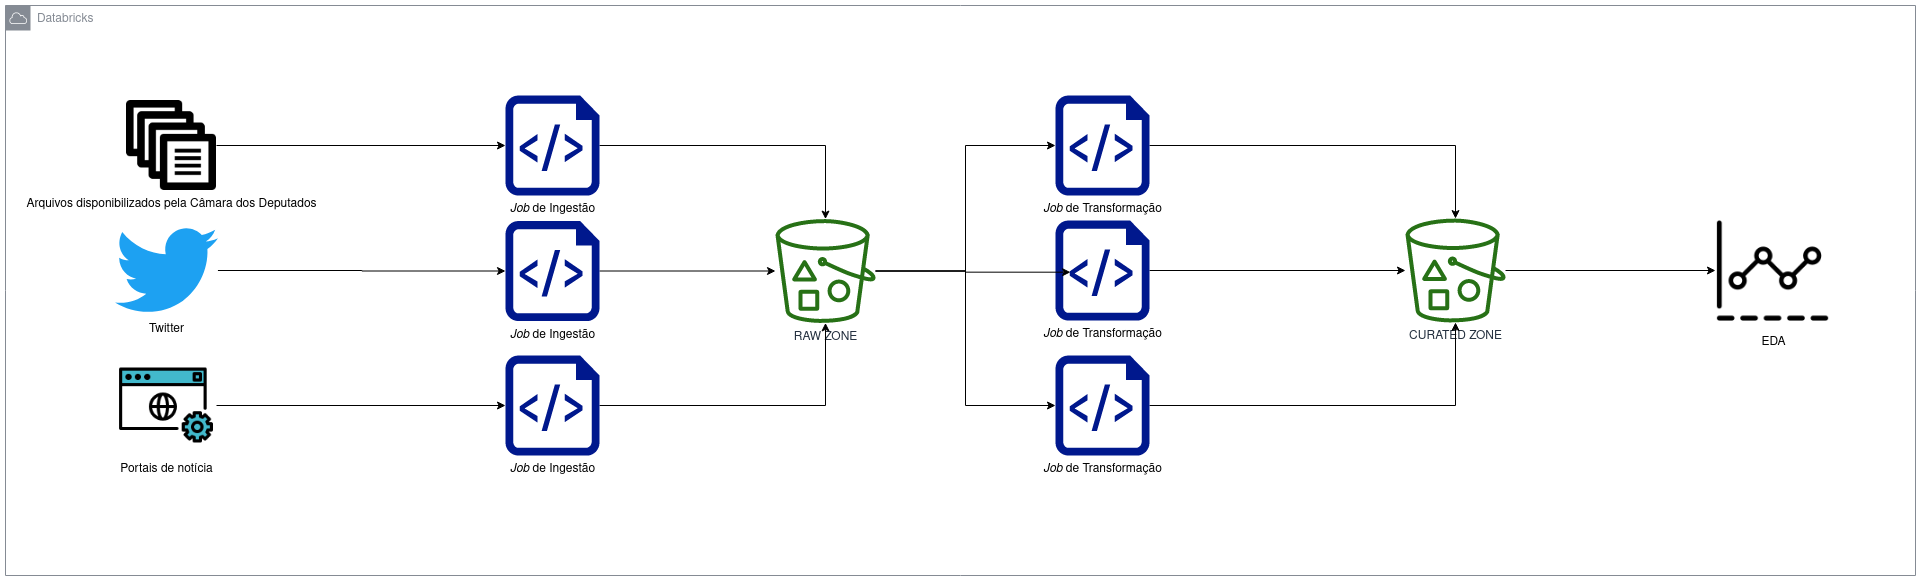
\includegraphics[width=.8\textwidth]{figuras/tcc_arch.png}
	% Caption centralizada
% 	\captionsetup{justification=centering}
	% Caption e fonte
	 \vspace{-0.3cm}
	\\\textbf{\footnotesize Fonte: Elaborada pelo autor}
	\label{fig:tela1}
\end{figure}

\section{Armazenamento} O Databricks está sendo utilizado como plataforma unificada do projeto, o que inclui o seu armazenamento. Uma das funcionalidades disponíveis é o \textit{file system} distribuído para armazenamento de dados em sua plataforma. É denominado como \textit{Databricks File System (DBFS)} e é compartilhado por todos os nós do \textit{cluster}\footnote{Disponível em <hhttps://docs.databricks.com/data/databricks-file-system.html> Acesso em: 19 mai, 2020}. Uma arquitetura de \textit{Data Lake} está sendo utilizada, logo temos a segmentação dos dados em zonas. Os dados originais são armazenados na \textit{Raw zone} em seu formato original. Após os processos de ETL, os dados já tratados são armazenados na \textit{Curated zone} em formato parquet, uma vez que este formato de armazenamento colunar é otimizado para o uso com o Spark e diminui drasticamente o espaço em disco necessário\footnote{Disponível em <https://parquet.apache.org/> Acesso em: 19 mai, 2020}.

\section{\textit{Extract, Transform and Load (ETL)}} Todo o processamento deste projeto foi realizado utilizando o Apache Spark. Este processamento foi segmentado em duas etapas, sendo elas:

\subsection{Ingestão de dados} Essa camada tem como objetivo o detalhamento dos processos que extraem os dados de sua fonte originária e os inserem, sem maiores tratamentos, no ambiente analítico. Foram elencadas 3 fontes de dados para o projeto, sendo elas:

\subsubsection{Dados Abertos da Câmara dos Deputados} A fonte oficial de dados da Câmara dos Deputados. Tratam-se de arquivos históricos disponibilizados pelo Câmara que contém todas as informações pessoais e políticas dos parlamentares, além dos históricos de reembolsos, discursos políticos, votações, emendas de sua autoria ou co-participação, entre diversas outras informações referentes à sua atividade parlamentar\footnote{Disponível em <https://dadosabertos.camara.leg.br/> Acesso em: 19 mai, 2020}. Os arquivos de 2009 a 2019 foram extraídos manualmente e inseridos na \textit{Raw zone} do nosso \textit{Data Lake}. Para este projeto, os dados dos seguintes temas foram extraídos:

\begin{itemize}
\item \textbf{Dados dos Deputados}: Deputados que já estiveram em exercício na Câmara dos Deputados;
\item \textbf{Despesas dos parlamentares}: Despesas referentes ao exercício da Atividade Parlamentar de cada deputado;
\item \textbf{Proposições}: Proposições apresentadas à Câmara dos Deputados com suas respectivas informações;
\item \textbf{Autores das Proposições}: Autores das proposições submetidas à Câmara;
\item \textbf{Classificação temática das proposições}: Informações mais detalhadas referentes aos temas das proposições submetidas.
\end{itemize}

\subsubsection{API do Twitter} O Twitter é uma rede social criada em 15 de julho de 2006 e, em fevereiro de 2019, possuia 321 milhões de usuários ativos\footnote{Disponível em <https://pt.wikipedia.org/wiki/Twitter> Acesso em: 19 mai, 2020}.Para extrair os \textit{tweets} desta plataforma, foi criado um \textit{job} utilizando Python e Spark e um módulo de comunicação com Twitter, o tweepy, que é caracterizado pelos autores como uma biblioteca de fácil uso para acesso à API do Twitter\footnote{Disponível em <https://www.tweepy.org/> Acesso em: 19 mai, 2020}. Para esse projeto, um arquivo com a listagem de todos os deputados e seus respectivos perfis oficiais no Twitter foi preenchido manualmente. Dessa forma, tornou-se possível a extração de todas as publicações de autoria dos parlamentares na plataforma.

\subsubsection{Portais de notícia} Se tratando dos portais de notícia, foi elencado o portal G1 como fonte de notícias políticas para alimentar o ambiente analítico. Para esse fim, um \textit{job} em Spark foi desenvolvido para realizar a extração das notícias políticas. Um filtro foi utilizado para extrair somente os artigos que tenham alguma referência aos parlamentares. 

\subsection{Transformação dos Dados} Nesta etapa, a limpeza e estruturação dos dados é realizada. Os dados armazenados na \textit{Raw zone} são utilizados como \textit{input} para essa camada da \textit{pipeline}. O processamento pode ser resumido na limpeza dos dados, filtro das informações e a estruturação das entidades para que a análise exploratória seja possível posteriormente. Após esse tratamento, os dados são armazenados em formato parquet na \textit{Curated zone}. Vários arquivos são escritos nessa zona em pastas, onde todos os arquivos desta pasta possuem o mesmo \textit{schema} e, utilizando o Spark SQL, este diretório é tratado como uma tabela em um banco de dados relacional. Temos um diretório para cada uma das seguintes entidades: autores das proposições, notícias, temas das proposições, proposições, contas do Twitter, \textit{tweets}, políticos e despesas. Pode-se observar a estrutura desta zona na figura 5.

% Figura
\begin{figure}[H]
	\centering	
	\caption[\hspace{0.1cm}Zona Curated]{\textit{Curated zone}}
	  \vspace{-0.4cm}
	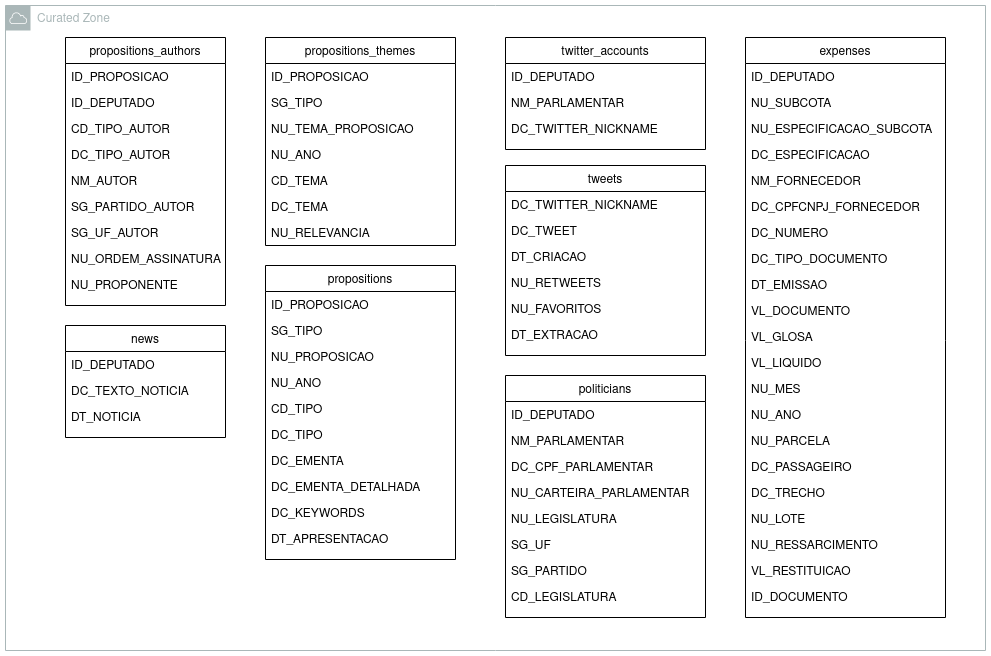
\includegraphics[width=.8\textwidth]{TCC/figuras/curated_zone.png}
	% Caption centralizada
% 	\captionsetup{justification=centering}
	% Caption e fonte
	 \vspace{-0.3cm}
	\\\textbf{\footnotesize Fonte: Elaborada pelo autor}
	\label{fig:tela1}
\end{figure}

Observa-se na figura 5 que todos os campos dos \textit{schemas} possuem um prefixo. Esse prefixo descreve a natureza do campo. Eles são definidos como: 

\begin{itemize}
\item \textbf{ID}: Identificador (inteiro);
\item \textbf{CD}: Código (\textit{string});
\item \textbf{DC}: Descrição (string);
\item \textbf{NM}: Nome (string);
\item \textbf{SG}: Sigla (string);
\item \textbf{NU}: Número (inteiro);
\item \textbf{VL}: Valor (decimal);
\item \textbf{DT}: Data (\textit{timestamp}).
\end{itemize}

\section{Análise exploratória de dados} Conforme descrito nas seções anteriores, todos os passos para extração e limpeza dos dados já foram realizados e, utilizando a \textit{Curated Zone}, os dados estão prontos para análise. Neste ponto, foram criados indicadores que descrevem as atividades parlamentares exercidas na Câmara dos Deputados, se tratando especificamente dos gastos dos parlamentares, os partidos políticos, proposições submetidas à Câmara com seus respectivos temas e status, além de categorizar as atividades dos políticos no Twitter e também as notícias que os citam no portal G1. Logo, tem-se um panorama geral onde pode-se identificar as reais atividades do deputado e compará-las com o seu discurso na mídia. Esse exercício comparativo foi realizado com uma amostra dos parlamentares existentes. Para essa análise, foram criadas 9 categorias, sendo elas: Cultura, Ciência, Trabalho, Saúde, Educação, Economia, Segurança Pública, Direitos Humanos e Desenvolvimento Urbano. Foram identificadas as proposições que possuem temas relacionados a essas categorias e também as atividades midiáticas dos parlamentares que se enquadram nesses grupos. Assim, um agrupamento foi realizado com granularidade a nível dos deputados contabilizando a quantidade de proposições e pronunciamentos para cada categoria, possibilitando a análise de correlação entre essas variáveis.
%\chapter{Desenvolvimento}
% Label para referenciar
%\label{desenvolvimento}

% Texto do capítulo

%Esta seção apresenta o desenvolvimento deste trabalho. Cada etapa da metodologia sera detalhada e apresentada atraves de seu codigo e observação

%\section{Classe utilitaria}

%Durante o desenvolvimento houve a necessidade de se criar um controle de versão dos arquivos para corrigir um problema de codificação do texto coletado do twitter devido a acentuação. Para controlar os arquivos de texto originais e traduzidos de cada candidato, foi criado uma classe utilitária denominada UTIL com dois atributos como podemos ver respectivamente nas linhas 2 e 3 , um foi utilizado para armazenar o nome do usuário do twitter e a outro em qual a versão dos arquivos se encontra. Assim esses atributos podem ser acessados de forma global por todas as outras classes do projeto, permitindo quando precisar criar um arquivo  daquele candidato.


%\section{Coleta de dados}

%O primeiro passo para o desenvolvimento do sistema foi a implementação da captura dos tweets do usuário que será submetido à análise. A captura foi realizada por meio da API disponibilizada pelo Twitter, utilizando o método \emph{GET statuses/user/timeline}, o qual retorna os 200 últimos \emph{tweets}. Esse valor é o maximo permitido por requicoes. Desta forma foi nessesario fazer uma nova requisiçao ja que 200 twitter nao é suficiente para uma analise confiavel.Podemos perceber que foi realizada uma requisição à API passando como parâmetro o último \emph{tweet} obtido pela primeira requisição. A segunda requisição coleta os próximos 200 \emph{tweets}. Apenas o texto com o conteúdo dos twittes do json retornado foi salvo no arquivo.

%O primeiro passo para o desenvolvimento do sistema foi a implementação da captura dos tweets do usuário que será submetido à análise. A captura foi realizada por meio da API disponibilizada pelo Twitter, utilizando o método \emph{GET statuses/user/timeline}, o qual retorna apenas os últimos  200 \emph{tweets}, esse e o valor máximo por cada requisição. Como esse valor e insuficiente para uma análise confiável foi feita uma nova chama ao método para coletar mais \emph{tweets} do usuário. Porem para isso é preciso passar como parâmetro na URL qual foi o último \emph{twitter} coletado para que a nova requisição traga apenas os \emph{twittes} que não foram coletados. Veja no Código 2.
%\begin{center}
%\begin{lstlisting}[title=Codigo 2 - Classe TwitterApi]
%class TwitterAPI:
%  def getTwitts(self):
%    session = OAuth1Session(self.CONSUMER_KEY, self.CONSUMER_SECRET, self.ACCESS_TOKEN_SECRET, self.ACCOUNT_ID)    
%    response = session.get('https://api.twitter.com/1.1/statuses/user_timeline.json?screen_name=' + Util.usuario + '&count=200')
%    tweets = json.loads(response.content)   
%    ultimo = tweets[len(tweets) -1]['id_str'].encode('utf-8')
%    arq = open(Util.usuario + Util.versao + '_PT-BR.txt', 'w')
%    linha = 0
%    while linha < len(tweets):
%      arq.write(tweets[linha]['text'].encode('utf-8') + "\n")
%      linha += 1
%    response = session.get('https://api.twitter.com/1.1/statuses/user_timeline.json?screen_name=' + Util.usuario + '&count=200&max_id=' + ultimo)
%    tweets = json.loads(response.content)
%   linha = 0
%    while linha < len(tweets):
%      arq.write(tweets[linha]['text'].encode('utf-8') + "\n")
%      linha += 1
%    arq.close()       
%\end{lstlisting}
%\textbf{\footnotesize Fonte: Criada pelo autor}
%\end{center}


%\section{Tradução do Texto}

%A segunda parte do desenvolvimento do código foi a implementação da tradução dos \emph{tweets} obtidos utilizando a API do Google Tradutor. Primeiramente o algoritimo lê o arquivo em Português e em seguida o envia para a API e salva o texto traduzido em um novo arquivo.

%A segunda parte do desenvolvimento do código foi a implementação da tradução dos \emph{tweets} . Foram testadas algumas Api gratuita porem todas tinha um limite caracteres ou por requisição ou cota diária o que todos eram insuficientes para este trabalho então foi utilizado a API  paga do Google Tradutor.

%Primeiramente o algoritmo lê o arquivo em Português daquele usuário e versão definida na classe UTIL. Em seguida o envia para a API através de uma requisição post onde é passado as chaves, qual é o idioma do texto original e do texto a ser traduzido como mostra a linha 2 do código 3. Após a resposta, o texto traduzido e salvo em um novo arquivo utilizando os padrões definidos.

%\begin{center}

%Antes de salvar o texto traduzido no arquivo, foi necessário converter sua codificação para UTF-8 para garantir que não haja problema com acentuação

%\section{Preparacao dos dados}

%Não foi preciso implementar, porque devido aos testes realizados durante o desenvolvimento, percebemos que a própria API do \emph{Personality Insight} não analisa os dados que ela não comprende.

%A terceira etapa do desenvolvimento definido na metodologia não foi precisa ser implementada, porque devido aos testes realizados durante o desenvolvimento e pesquisas feitas sobre o algoritmo utilizado no \emph{Personality Insight} as palavras que não se encontra no dicionário da língua inglesa não são consideradas na avaliação do perfil. 

%\section{API Personality Insight}

%A Classe Personality Insight apresenta o método que realiza a requição ao \emph{Bluemix} para a análise de personalidade. A API exige que seja enviado um \emph{profile} contendo o texto a ser analisado, qual idioma deseja obter os resultados, entre outras informaçoes opcionais. A API retorna um JSON com todos os resultados, que serão salvos em um outro arquivo de texto.

%No último método novamente lemos um arquivo porem dessa vez o que possui o texto em inglês e em seguida é feito a requisição a ao Personality Insight. A api da ibm  e precisa ser configurada com os parâmetro da versão a ser utilizada no caso foi a v3, a última já desenvolvida, além do usuário e senha do desenvolvedor no  Bluemix . Já a requisição e feita através do método profile que recebe o texto em inglês a ser analisado, o formato dele, quais serão os resultados retornados, e o idioma de saída no caso português do Brasil. Após a requisição a resposta e salva no formato json original com todos os dados obtidos em um outro arquivo com o mesmo nome de usuário e versão dos arquivos de texto português e inglês.


%\section{Correlação dos resultados dos testes}

%\begin{table}[H]
%\centering
%\caption{My Personality 100-item x Personality Insight }
%\label{Correlação Candidato 1}
%\resizebox{\textwidth}{!}{%
%\begin{tabular}{@{}cccc@{}}
%\toprule
%Candidato & Correlação   \\ \midrule
%Candidato 1 & 0,42 &  \\
%Candidato 2  & 0,28 \\
%Candidato 3  & 0,36 \\
 %\bottomrule
%\end{tabular}%
%}
%\end{table}

\chapter{Resultados}
% Label para referenciar
\label{resultados}

\section{Análise explorátoria de dados} Na etapa de \ac{EDA}, utilizando os dados que foram tratados e armazenados nas etapas anteriores, será possível iniciar as análises estatísticas com o intuito de entender as distribuições, padrões e correlações existentes na massa de dados do \textit{Data Lake}. É uma etapa fundamental do processo, uma vez que é nessa etapa que o conhecimento é efetivamente gerado. Temos o objetivo de possibilitar a análise da atividade política de cada parlamentar de Câmara dos Deputados Federal a partir de dados oficiais, possibilitando uma visão clara e objetiva de gastos incomuns, quais os termos mais utilizados, 

\chapter{Conclusão}
% Label para referenciar
\label{conclusão}
O objetivo geral desse trabalho foi...


 \section{Trabalhos futuros}
Como trabalhos futuros, pode-se apontar:
  

% ----------------------------------------------------------



% ----------------------------------------------------------
% Finaliza a parte no bookmark do PDF
% para que se inicie o bookmark na raiz
% e adiciona espaço de parte no Sumário
% ----------------------------------------------------------
\phantompart

% ---
% Conclusão
% ---
%\chapter{Conclusão}
% Label para referenciar
\label{conclusão}
O objetivo geral desse trabalho foi...


 \section{Trabalhos futuros}
Como trabalhos futuros, pode-se apontar:
  

% ---

% ----------------------------------------------------------
% ELEMENTOS PÓS-TEXTUAIS
% ----------------------------------------------------------
\postextual
% ----------------------------------------------------------

% ----------------------------------------------------------
% Referências bibliográficas
% ----------------------------------------------------------
\bibliography{bibliografia}

% ----------------------------------------------------------
% Glossário
% ----------------------------------------------------------
%
% Consulte o manual da classe abntex2 para orientações sobre o glossário.
%
%\glossary

% ----------------------------------------------------------
% Apêndices
% ----------------------------------------------------------

% ---
% Inicia os apêndices
% \partapendices -- Imprime uma página indicando o início dos apêndices
% ---

%\begin{apendicesenv}
%\partapendices
%\chapter{Gráficos de resultados complementares}
\label{apendice}


Neste apêndice, apresenta-se figuras complementares àquelas apresentadas durante o desenvolvimento dos resultados desse trabalho. Tratam-se de gráficos com mais detalhes dos resultados, incluindo os valores obtidos da pesquisa.

%%%%%%%%% CG

\begin{figure}[htb] 
	\caption{Aplicação CG - Topologia M-0} \centering
  \subfloat[Tempo simulado]    {\label{graf:cg:m0:sim_seconds}\includegraphics[width=.45\textwidth]{imagem/graficos/sim_seconds/CG_M-0.pdf}}
  \subfloat[Latência da rede]  {\label{graf:cg:m0:net_latency}\includegraphics[width=.45\textwidth]{imagem/graficos/net_latency/CG_M-0.pdf}} \quad
  \subfloat[Potência consumida]{\label{graf:cg:m0:noc_power}  \includegraphics[width=.45\textwidth]  {imagem/graficos/noc_power/CG_M-0.pdf}}
	\subfloat[Taxa de faltas]    {\label{graf:cg:m0:avg_l2_miss}\includegraphics[width=.45\textwidth]{imagem/graficos/avg_l2_miss/CG_M-0.pdf}}
	\legend{Fonte: Dados da pesquisa}	\label{graf:cg:m0}
\end{figure}
\begin{figure}[htb] 
    \caption{Aplicação CG - Topologia M1} \centering
  \subfloat[Tempo simulado]    {\label{graf:cg:m1:sim_seconds}\includegraphics[width=.45\textwidth]{imagem/graficos/sim_seconds/CG_M-1.pdf}}
  \subfloat[Latência da rede]  {\label{graf:cg:m1:net_latency}\includegraphics[width=.45\textwidth]{imagem/graficos/net_latency/CG_M-1.pdf}} \quad
  \subfloat[Potência consumida]{\label{graf:cg:m1:noc_power}  \includegraphics[width=.45\textwidth]  {imagem/graficos/noc_power/CG_M-1.pdf}}
	\subfloat[Taxa de faltas]    {\label{graf:cg:m1:avg_l2_miss}\includegraphics[width=.45\textwidth]{imagem/graficos/avg_l2_miss/CG_M-1.pdf}}
	\legend{Fonte: Dados da pesquisa}	\label{graf:cg:m1}
\end{figure}
\begin{figure}[htb] \setlength{\abovecaptionskip}{-2pt}
    \caption{Aplicação CG - Topologia M2} \centering
  \subfloat[Tempo simulado]    {\label{graf:cg:m2:sim_seconds}\includegraphics[width=.45\textwidth]{imagem/graficos/sim_seconds/CG_M-2.pdf}}
  \subfloat[Latência da rede]  {\label{graf:cg:m2:net_latency}\includegraphics[width=.45\textwidth]{imagem/graficos/net_latency/CG_M-2.pdf}} \quad
  \subfloat[Potência consumida]{\label{graf:cg:m2:noc_power}  \includegraphics[width=.45\textwidth]  {imagem/graficos/noc_power/CG_M-2.pdf}}
	\subfloat[Taxa de faltas]    {\label{graf:cg:m2:avg_l2_miss}\includegraphics[width=.45\textwidth]{imagem/graficos/avg_l2_miss/CG_M-2.pdf}}
	\legend{Fonte: Dados da pesquisa}	\label{graf:cg:m2}
\end{figure}
\begin{figure}[htb] 
    \caption{Aplicação CG - Topologia M3} \centering
  \subfloat[Tempo simulado]    {\label{graf:cg:m3:sim_seconds}\includegraphics[width=.45\textwidth]{imagem/graficos/sim_seconds/CG_M-3.pdf}}
  \subfloat[Latência da rede]  {\label{graf:cg:m3:net_latency}\includegraphics[width=.45\textwidth]{imagem/graficos/net_latency/CG_M-3.pdf}} \quad
  \subfloat[Potência consumida]{\label{graf:cg:m3:noc_power}  \includegraphics[width=.45\textwidth]  {imagem/graficos/noc_power/CG_M-3.pdf}}
	\subfloat[Taxa de faltas]    {\label{graf:cg:m3:avg_l2_miss}\includegraphics[width=.45\textwidth]{imagem/graficos/avg_l2_miss/CG_M-3.pdf}}
	\legend{Fonte: Dados da pesquisa}	\label{graf:cg:m3}
\end{figure}
\begin{figure}[htb] 
    \caption{Aplicação CG - Topologia M4} \centering
  \subfloat[Tempo simulado]    {\label{graf:cg:m4:sim_seconds}\includegraphics[width=.45\textwidth]{imagem/graficos/sim_seconds/CG_M-4.pdf}}
  \subfloat[Latência da rede]  {\label{graf:cg:m4:net_latency}\includegraphics[width=.45\textwidth]{imagem/graficos/net_latency/CG_M-4.pdf}} \quad
  \subfloat[Potência consumida]{\label{graf:cg:m4:noc_power}  \includegraphics[width=.45\textwidth]  {imagem/graficos/noc_power/CG_M-4.pdf}}
	\subfloat[Taxa de faltas]    {\label{graf:cg:m4:avg_l2_miss}\includegraphics[width=.45\textwidth]{imagem/graficos/avg_l2_miss/CG_M-4.pdf}}
	\legend{Fonte: Dados da pesquisa}	\label{graf:cg:m4}
\end{figure}
\begin{figure}[H] \setlength{\abovecaptionskip}{-2pt} \setlength{\belowcaptionskip}{0pt} \captionsetup[subfloat]{captionskip=-10pt}
  \caption{Aplicação CG - Topologia T1} \centering
  \subfloat[Tempo simulado]    {\label{graf:cg:t1:sim_seconds}\includegraphics[width=.45\textwidth]{imagem/graficos/sim_seconds/CG_T-1.pdf}}
  \subfloat[Latência da rede]  {\label{graf:cg:t1:net_latency}\includegraphics[width=.45\textwidth]{imagem/graficos/net_latency/CG_T-1.pdf}} \quad
  \subfloat[Potência consumida]{\label{graf:cg:t1:noc_power}  \includegraphics[width=.45\textwidth]  {imagem/graficos/noc_power/CG_T-1.pdf}}
	\subfloat[Taxa de faltas]    {\label{graf:cg:t1:avg_l2_miss}\includegraphics[width=.45\textwidth]{imagem/graficos/avg_l2_miss/CG_T-1.pdf}}
	\captionsetup{justification=centering} \captionfont{\small{\textbf{\\Fonte: Dados da pesquisa}}}	\label{graf:cg:t1}
\end{figure}
\begin{figure}[H] \setlength{\abovecaptionskip}{-2pt} \setlength{\belowcaptionskip}{0pt} \captionsetup[subfloat]{captionskip=-10pt}
  \caption{Aplicação CG - Topologia T2} \centering
  \subfloat[Tempo simulado]    {\label{graf:cg:t2:sim_seconds}\includegraphics[width=.45\textwidth]{imagem/graficos/sim_seconds/CG_T-2.pdf}}
  \subfloat[Latência da rede]  {\label{graf:cg:t2:net_latency}\includegraphics[width=.45\textwidth]{imagem/graficos/net_latency/CG_T-2.pdf}} \quad
  \subfloat[Potência consumida]{\label{graf:cg:t2:noc_power}  \includegraphics[width=.45\textwidth]  {imagem/graficos/noc_power/CG_T-2.pdf}}
	\subfloat[Taxa de faltas]    {\label{graf:cg:t2:avg_l2_miss}\includegraphics[width=.45\textwidth]{imagem/graficos/avg_l2_miss/CG_T-2.pdf}}
	\captionsetup{justification=centering} \captionfont{\small{\textbf{\\Fonte: Dados da pesquisa}}}	\label{graf:cg:t2}
\end{figure}
\begin{figure}[H] \setlength{\abovecaptionskip}{-2pt} \setlength{\belowcaptionskip}{0pt} \captionsetup[subfloat]{captionskip=-10pt}
  \caption{Aplicação CG - Topologia T3} \centering
  \subfloat[Tempo simulado]    {\label{graf:cg:t3:sim_seconds}\includegraphics[width=.45\textwidth]{imagem/graficos/sim_seconds/CG_T-3.pdf}}
  \subfloat[Latência da rede]  {\label{graf:cg:t3:net_latency}\includegraphics[width=.45\textwidth]{imagem/graficos/net_latency/CG_T-3.pdf}} \quad
  \subfloat[Potência consumida]{\label{graf:cg:t3:noc_power}  \includegraphics[width=.45\textwidth]  {imagem/graficos/noc_power/CG_T-3.pdf}}
	\subfloat[Taxa de faltas]    {\label{graf:cg:t3:avg_l2_miss}\includegraphics[width=.45\textwidth]{imagem/graficos/avg_l2_miss/CG_T-3.pdf}}
	\captionsetup{justification=centering} \captionfont{\small{\textbf{\\Fonte: Dados da pesquisa}}}	\label{graf:cg:t3}
\end{figure}
\begin{figure}[H] \setlength{\abovecaptionskip}{-2pt} \setlength{\belowcaptionskip}{0pt} \captionsetup[subfloat]{captionskip=-10pt}
  \caption{Aplicação CG - Topologia T4} \centering
  \subfloat[Tempo simulado]    {\label{graf:cg:t4:sim_seconds}\includegraphics[width=.45\textwidth]{imagem/graficos/sim_seconds/CG_T-4.pdf}}
  \subfloat[Latência da rede]  {\label{graf:cg:t4:net_latency}\includegraphics[width=.45\textwidth]{imagem/graficos/net_latency/CG_T-4.pdf}} \quad
  \subfloat[Potência consumida]{\label{graf:cg:t4:noc_power}  \includegraphics[width=.45\textwidth]  {imagem/graficos/noc_power/CG_T-4.pdf}}
	\subfloat[Taxa de faltas]    {\label{graf:cg:t4:avg_l2_miss}\includegraphics[width=.45\textwidth]{imagem/graficos/avg_l2_miss/CG_T-4.pdf}}
	\captionsetup{justification=centering} \captionfont{\small{\textbf{\\Fonte: Dados da pesquisa}}}	\label{graf:cg:t4}
\end{figure}
\begin{figure}[H] \setlength{\abovecaptionskip}{-2pt} \setlength{\belowcaptionskip}{0pt} \captionsetup[subfloat]{captionskip=-10pt}
  \caption{Aplicação CG - Topologia C4} \centering
  \subfloat[Tempo simulado]    {\label{graf:cg:c4:sim_seconds}\includegraphics[width=.45\textwidth]{imagem/graficos/sim_seconds/CG_C-4.pdf}}
  \subfloat[Latência da rede]  {\label{graf:cg:c4:net_latency}\includegraphics[width=.45\textwidth]{imagem/graficos/net_latency/CG_C-4.pdf}} \quad
  \subfloat[Potência consumida]{\label{graf:cg:c4:noc_power}  \includegraphics[width=.45\textwidth]  {imagem/graficos/noc_power/CG_C-4.pdf}}
	\subfloat[Taxa de faltas]    {\label{graf:cg:c4:avg_l2_miss}\includegraphics[width=.45\textwidth]{imagem/graficos/avg_l2_miss/CG_C-4.pdf}}
	\captionsetup{justification=centering} \captionfont{\small{\textbf{\\Fonte: Dados da pesquisa}}}	\label{graf:cg:c4}
\end{figure}
\begin{figure}[H] \setlength{\abovecaptionskip}{-2pt} \setlength{\belowcaptionskip}{0pt} \captionsetup[subfloat]{captionskip=-10pt}
  \caption{Aplicação CG - Topologia C8} \centering
  \subfloat[Tempo simulado]    {\label{graf:cg:c8:sim_seconds}\includegraphics[width=.45\textwidth]{imagem/graficos/sim_seconds/CG_C-8.pdf}}
  \subfloat[Latência da rede]  {\label{graf:cg:c8:net_latency}\includegraphics[width=.45\textwidth]{imagem/graficos/net_latency/CG_C-8.pdf}} \quad
  \subfloat[Potência consumida]{\label{graf:cg:c8:noc_power}  \includegraphics[width=.45\textwidth]  {imagem/graficos/noc_power/CG_C-8.pdf}}
	\subfloat[Taxa de faltas]    {\label{graf:cg:c8:avg_l2_miss}\includegraphics[width=.45\textwidth]{imagem/graficos/avg_l2_miss/CG_C-8.pdf}}
	\captionsetup{justification=centering} \captionfont{\small{\textbf{\\Fonte: Dados da pesquisa}}}	\label{graf:cg:c8}
\end{figure}
\begin{figure}[H] \setlength{\abovecaptionskip}{-2pt} \setlength{\belowcaptionskip}{0pt} \captionsetup[subfloat]{captionskip=-10pt}
  \caption{Aplicação CG - Topologia C16} \centering
  \subfloat[Tempo simulado]    {\label{graf:cg:c16:sim_seconds}\includegraphics[width=.45\textwidth]{imagem/graficos/sim_seconds/CG_C-16.pdf}}
  \subfloat[Latência da rede]  {\label{graf:cg:c16:net_latency}\includegraphics[width=.45\textwidth]{imagem/graficos/net_latency/CG_C-16.pdf}} \quad
  \subfloat[Potência consumida]{\label{graf:cg:c16:noc_power}  \includegraphics[width=.45\textwidth]  {imagem/graficos/noc_power/CG_C-16.pdf}}
	\subfloat[Taxa de faltas]    {\label{graf:cg:c16:avg_l2_miss}\includegraphics[width=.45\textwidth]{imagem/graficos/avg_l2_miss/CG_C-16.pdf}}
	\captionsetup{justification=centering} \captionfont{\small{\textbf{\\Fonte: Dados da pesquisa}}}	\label{graf:cg:c16}
\end{figure}


%%%%%%%%% EP
\begin{figure}[H] \setlength{\abovecaptionskip}{-2pt} \setlength{\belowcaptionskip}{0pt} \captionsetup[subfloat]{captionskip=-10pt}
  \caption{Aplicação EP - Topologia M-0} \centering
  \subfloat[Tempo simulado]    {\label{graf:ep:m0:sim_seconds}\includegraphics[width=.45\textwidth]{imagem/graficos/sim_seconds/EP_M-0.pdf}}
  \subfloat[Latência da rede]  {\label{graf:ep:m0:net_latency}\includegraphics[width=.45\textwidth]{imagem/graficos/net_latency/EP_M-0.pdf}} \quad
  \subfloat[Potência consumida]{\label{graf:ep:m0:noc_power}  \includegraphics[width=.45\textwidth]  {imagem/graficos/noc_power/EP_M-0.pdf}}
	\subfloat[Taxa de faltas]    {\label{graf:ep:m0:avg_l2_miss}\includegraphics[width=.45\textwidth]{imagem/graficos/avg_l2_miss/EP_M-0.pdf}}
	\captionsetup{justification=centering} \captionfont{\small{\textbf{\\Fonte: Dados da pesquisa}}}	\label{graf:ep:m0}
\end{figure}
\begin{figure}[H] \setlength{\abovecaptionskip}{-2pt} \setlength{\belowcaptionskip}{0pt} \captionsetup[subfloat]{captionskip=-10pt}
  \caption{Aplicação EP - Topologia M1} \centering
  \subfloat[Tempo simulado]    {\label{graf:ep:m1:sim_seconds}\includegraphics[width=.45\textwidth]{imagem/graficos/sim_seconds/EP_M-1.pdf}}
  \subfloat[Latência da rede]  {\label{graf:ep:m1:net_latency}\includegraphics[width=.45\textwidth]{imagem/graficos/net_latency/EP_M-1.pdf}} \quad
  \subfloat[Potência consumida]{\label{graf:ep:m1:noc_power}  \includegraphics[width=.45\textwidth]  {imagem/graficos/noc_power/EP_M-1.pdf}}
	\subfloat[Taxa de faltas]    {\label{graf:ep:m1:avg_l2_miss}\includegraphics[width=.45\textwidth]{imagem/graficos/avg_l2_miss/EP_M-1.pdf}}
	\captionsetup{justification=centering} \captionfont{\small{\textbf{\\Fonte: Dados da pesquisa}}}	\label{graf:ep:m1}
\end{figure}
\begin{figure}[H] \setlength{\abovecaptionskip}{-2pt} \setlength{\belowcaptionskip}{0pt} \captionsetup[subfloat]{captionskip=-10pt}
  \caption{Aplicação EP - Topologia M2} \centering
  \subfloat[Tempo simulado]    {\label{graf:ep:m2:sim_seconds}\includegraphics[width=.45\textwidth]{imagem/graficos/sim_seconds/EP_M-2.pdf}}
  \subfloat[Latência da rede]  {\label{graf:ep:m2:net_latency}\includegraphics[width=.45\textwidth]{imagem/graficos/net_latency/EP_M-2.pdf}} \quad
  \subfloat[Potência consumida]{\label{graf:ep:m2:noc_power}  \includegraphics[width=.45\textwidth]  {imagem/graficos/noc_power/EP_M-2.pdf}}
	\subfloat[Taxa de faltas]    {\label{graf:ep:m2:avg_l2_miss}\includegraphics[width=.45\textwidth]{imagem/graficos/avg_l2_miss/EP_M-2.pdf}}
	\captionsetup{justification=centering} \captionfont{\small{\textbf{\\Fonte: Dados da pesquisa}}}	\label{graf:ep:m2}
\end{figure}
\begin{figure}[H] \setlength{\abovecaptionskip}{-2pt} \setlength{\belowcaptionskip}{0pt} \captionsetup[subfloat]{captionskip=-10pt}
  \caption{Aplicação EP - Topologia M3} \centering
  \subfloat[Tempo simulado]    {\label{graf:ep:m3:sim_seconds}\includegraphics[width=.45\textwidth]{imagem/graficos/sim_seconds/EP_M-3.pdf}}
  \subfloat[Latência da rede]  {\label{graf:ep:m3:net_latency}\includegraphics[width=.45\textwidth]{imagem/graficos/net_latency/EP_M-3.pdf}} \quad
  \subfloat[Potência consumida]{\label{graf:ep:m3:noc_power}  \includegraphics[width=.45\textwidth]  {imagem/graficos/noc_power/EP_M-3.pdf}}
	\subfloat[Taxa de faltas]    {\label{graf:ep:m3:avg_l2_miss}\includegraphics[width=.45\textwidth]{imagem/graficos/avg_l2_miss/EP_M-3.pdf}}
	\captionsetup{justification=centering} \captionfont{\small{\textbf{\\Fonte: Dados da pesquisa}}}	\label{graf:ep:m3}
\end{figure}
\begin{figure}[H] \setlength{\abovecaptionskip}{-2pt} \setlength{\belowcaptionskip}{0pt} \captionsetup[subfloat]{captionskip=-10pt}
  \caption{Aplicação EP - Topologia M4} \centering
  \subfloat[Tempo simulado]    {\label{graf:ep:m4:sim_seconds}\includegraphics[width=.45\textwidth]{imagem/graficos/sim_seconds/EP_M-4.pdf}}
  \subfloat[Latência da rede]  {\label{graf:ep:m4:net_latency}\includegraphics[width=.45\textwidth]{imagem/graficos/net_latency/EP_M-4.pdf}} \quad
  \subfloat[Potência consumida]{\label{graf:ep:m4:noc_power}  \includegraphics[width=.45\textwidth]  {imagem/graficos/noc_power/EP_M-4.pdf}}
	\subfloat[Taxa de faltas]    {\label{graf:ep:m4:avg_l2_miss}\includegraphics[width=.45\textwidth]{imagem/graficos/avg_l2_miss/EP_M-4.pdf}}
	\captionsetup{justification=centering} \captionfont{\small{\textbf{\\Fonte: Dados da pesquisa}}}	\label{graf:ep:m4}
\end{figure}
\begin{figure}[H] \setlength{\abovecaptionskip}{-2pt} \setlength{\belowcaptionskip}{0pt} \captionsetup[subfloat]{captionskip=-10pt}
  \caption{Aplicação EP - Topologia T1} \centering
  \subfloat[Tempo simulado]    {\label{graf:ep:t1:sim_seconds}\includegraphics[width=.45\textwidth]{imagem/graficos/sim_seconds/EP_T-1.pdf}}
  \subfloat[Latência da rede]  {\label{graf:ep:t1:net_latency}\includegraphics[width=.45\textwidth]{imagem/graficos/net_latency/EP_T-1.pdf}} \quad
  \subfloat[Potência consumida]{\label{graf:ep:t1:noc_power}  \includegraphics[width=.45\textwidth]  {imagem/graficos/noc_power/EP_T-1.pdf}}
	\subfloat[Taxa de faltas]    {\label{graf:ep:t1:avg_l2_miss}\includegraphics[width=.45\textwidth]{imagem/graficos/avg_l2_miss/EP_T-1.pdf}}
	\captionsetup{justification=centering} \captionfont{\small{\textbf{\\Fonte: Dados da pesquisa}}}	\label{graf:ep:t1}
\end{figure}
\begin{figure}[H] \setlength{\abovecaptionskip}{-2pt} \setlength{\belowcaptionskip}{0pt} \captionsetup[subfloat]{captionskip=-10pt}
  \caption{Aplicação EP - Topologia T2} \centering
  \subfloat[Tempo simulado]    {\label{graf:ep:t2:sim_seconds}\includegraphics[width=.45\textwidth]{imagem/graficos/sim_seconds/EP_T-2.pdf}}
  \subfloat[Latência da rede]  {\label{graf:ep:t2:net_latency}\includegraphics[width=.45\textwidth]{imagem/graficos/net_latency/EP_T-2.pdf}} \quad
  \subfloat[Potência consumida]{\label{graf:ep:t2:noc_power}  \includegraphics[width=.45\textwidth]  {imagem/graficos/noc_power/EP_T-2.pdf}}
	\subfloat[Taxa de faltas]    {\label{graf:ep:t2:avg_l2_miss}\includegraphics[width=.45\textwidth]{imagem/graficos/avg_l2_miss/EP_T-2.pdf}}
	\captionsetup{justification=centering} \captionfont{\small{\textbf{\\Fonte: Dados da pesquisa}}}	\label{graf:ep:t2}
\end{figure}
\begin{figure}[H] \setlength{\abovecaptionskip}{-2pt} \setlength{\belowcaptionskip}{0pt} \captionsetup[subfloat]{captionskip=-10pt}
  \caption{Aplicação EP - Topologia T3} \centering
  \subfloat[Tempo simulado]    {\label{graf:ep:t3:sim_seconds}\includegraphics[width=.45\textwidth]{imagem/graficos/sim_seconds/EP_T-3.pdf}}
  \subfloat[Latência da rede]  {\label{graf:ep:t3:net_latency}\includegraphics[width=.45\textwidth]{imagem/graficos/net_latency/EP_T-3.pdf}} \quad
  \subfloat[Potência consumida]{\label{graf:ep:t3:noc_power}  \includegraphics[width=.45\textwidth]  {imagem/graficos/noc_power/EP_T-3.pdf}}
	\subfloat[Taxa de faltas]    {\label{graf:ep:t3:avg_l2_miss}\includegraphics[width=.45\textwidth]{imagem/graficos/avg_l2_miss/EP_T-3.pdf}}
	\captionsetup{justification=centering} \captionfont{\small{\textbf{\\Fonte: Dados da pesquisa}}}	\label{graf:ep:t3}
\end{figure}
\begin{figure}[H] \setlength{\abovecaptionskip}{-2pt} \setlength{\belowcaptionskip}{0pt} \captionsetup[subfloat]{captionskip=-10pt}
  \caption{Aplicação EP - Topologia T4} \centering
  \subfloat[Tempo simulado]    {\label{graf:ep:t4:sim_seconds}\includegraphics[width=.45\textwidth]{imagem/graficos/sim_seconds/EP_T-4.pdf}}
  \subfloat[Latência da rede]  {\label{graf:ep:t4:net_latency}\includegraphics[width=.45\textwidth]{imagem/graficos/net_latency/EP_T-4.pdf}} \quad
  \subfloat[Potência consumida]{\label{graf:ep:t4:noc_power}  \includegraphics[width=.45\textwidth]  {imagem/graficos/noc_power/EP_T-4.pdf}}
	\subfloat[Taxa de faltas]    {\label{graf:ep:t4:avg_l2_miss}\includegraphics[width=.45\textwidth]{imagem/graficos/avg_l2_miss/EP_T-4.pdf}}
	\captionsetup{justification=centering} \captionfont{\small{\textbf{\\Fonte: Dados da pesquisa}}}	\label{graf:ep:t4}
\end{figure}
\begin{figure}[H] \setlength{\abovecaptionskip}{-2pt} \setlength{\belowcaptionskip}{0pt} \captionsetup[subfloat]{captionskip=-10pt}
  \caption{Aplicação EP - Topologia C4} \centering
  \subfloat[Tempo simulado]    {\label{graf:ep:c4:sim_seconds}\includegraphics[width=.45\textwidth]{imagem/graficos/sim_seconds/EP_C-4.pdf}}
  \subfloat[Latência da rede]  {\label{graf:ep:c4:net_latency}\includegraphics[width=.45\textwidth]{imagem/graficos/net_latency/EP_C-4.pdf}} \quad
  \subfloat[Potência consumida]{\label{graf:ep:c4:noc_power}  \includegraphics[width=.45\textwidth]  {imagem/graficos/noc_power/EP_C-4.pdf}}
	\subfloat[Taxa de faltas]    {\label{graf:ep:c4:avg_l2_miss}\includegraphics[width=.45\textwidth]{imagem/graficos/avg_l2_miss/EP_C-4.pdf}}
	\captionsetup{justification=centering} \captionfont{\small{\textbf{\\Fonte: Dados da pesquisa}}}	\label{graf:ep:c4}
\end{figure}
\begin{figure}[H] \setlength{\abovecaptionskip}{-2pt} \setlength{\belowcaptionskip}{0pt} \captionsetup[subfloat]{captionskip=-10pt}
  \caption{Aplicação EP - Topologia C8} \centering
  \subfloat[Tempo simulado]    {\label{graf:ep:c8:sim_seconds}\includegraphics[width=.45\textwidth]{imagem/graficos/sim_seconds/EP_C-8.pdf}}
  \subfloat[Latência da rede]  {\label{graf:ep:c8:net_latency}\includegraphics[width=.45\textwidth]{imagem/graficos/net_latency/EP_C-8.pdf}} \quad
  \subfloat[Potência consumida]{\label{graf:ep:c8:noc_power}  \includegraphics[width=.45\textwidth]  {imagem/graficos/noc_power/EP_C-8.pdf}}
	\subfloat[Taxa de faltas]    {\label{graf:ep:c8:avg_l2_miss}\includegraphics[width=.45\textwidth]{imagem/graficos/avg_l2_miss/EP_C-8.pdf}}
	\captionsetup{justification=centering} \captionfont{\small{\textbf{\\Fonte: Dados da pesquisa}}}	\label{graf:ep:c8}
\end{figure}

%%%%%%%%% FT
\begin{figure}[H] \setlength{\abovecaptionskip}{-2pt} \setlength{\belowcaptionskip}{0pt} \captionsetup[subfloat]{captionskip=-10pt}
  \caption{Aplicação FT - Topologia M-0} \centering
  \subfloat[Tempo simulado]    {\label{graf:ft:m0:sim_seconds}\includegraphics[width=.45\textwidth]{imagem/graficos/sim_seconds/FT_M-0.pdf}}
  \subfloat[Latência da rede]  {\label{graf:ft:m0:net_latency}\includegraphics[width=.45\textwidth]{imagem/graficos/net_latency/FT_M-0.pdf}} \quad
  \subfloat[Potência consumida]{\label{graf:ft:m0:noc_power}  \includegraphics[width=.45\textwidth]  {imagem/graficos/noc_power/FT_M-0.pdf}}
	\subfloat[Taxa de faltas]    {\label{graf:ft:m0:avg_l2_miss}\includegraphics[width=.45\textwidth]{imagem/graficos/avg_l2_miss/FT_M-0.pdf}}
	\captionsetup{justification=centering} \captionfont{\small{\textbf{\\Fonte: Dados da pesquisa}}}	\label{graf:ft:m0}
\end{figure}
\begin{figure}[H] \setlength{\abovecaptionskip}{-2pt} \setlength{\belowcaptionskip}{0pt} \captionsetup[subfloat]{captionskip=-10pt}
  \caption{Aplicação FT - Topologia M1} \centering
  \subfloat[Tempo simulado]    {\label{graf:ft:m1:sim_seconds}\includegraphics[width=.45\textwidth]{imagem/graficos/sim_seconds/FT_M-1.pdf}}
  \subfloat[Latência da rede]  {\label{graf:ft:m1:net_latency}\includegraphics[width=.45\textwidth]{imagem/graficos/net_latency/FT_M-1.pdf}} \quad
  \subfloat[Potência consumida]{\label{graf:ft:m1:noc_power}  \includegraphics[width=.45\textwidth]  {imagem/graficos/noc_power/FT_M-1.pdf}}
	\subfloat[Taxa de faltas]    {\label{graf:ft:m1:avg_l2_miss}\includegraphics[width=.45\textwidth]{imagem/graficos/avg_l2_miss/FT_M-1.pdf}}
	\captionsetup{justification=centering} \captionfont{\small{\textbf{\\Fonte: Dados da pesquisa}}}	\label{graf:ft:m1}
\end{figure}
\begin{figure}[H] \setlength{\abovecaptionskip}{-2pt} \setlength{\belowcaptionskip}{0pt} \captionsetup[subfloat]{captionskip=-10pt}
  \caption{Aplicação FT - Topologia M2} \centering
  \subfloat[Tempo simulado]    {\label{graf:ft:m2:sim_seconds}\includegraphics[width=.45\textwidth]{imagem/graficos/sim_seconds/FT_M-2.pdf}}
  \subfloat[Latência da rede]  {\label{graf:ft:m2:net_latency}\includegraphics[width=.45\textwidth]{imagem/graficos/net_latency/FT_M-2.pdf}} \quad
  \subfloat[Potência consumida]{\label{graf:ft:m2:noc_power}  \includegraphics[width=.45\textwidth]  {imagem/graficos/noc_power/FT_M-2.pdf}}
	\subfloat[Taxa de faltas]    {\label{graf:ft:m2:avg_l2_miss}\includegraphics[width=.45\textwidth]{imagem/graficos/avg_l2_miss/FT_M-2.pdf}}
	\captionsetup{justification=centering} \captionfont{\small{\textbf{\\Fonte: Dados da pesquisa}}}	\label{graf:ft:m2}
\end{figure}
\begin{figure}[H] \setlength{\abovecaptionskip}{-2pt} \setlength{\belowcaptionskip}{0pt} \captionsetup[subfloat]{captionskip=-10pt}
  \caption{Aplicação FT - Topologia M3} \centering
  \subfloat[Tempo simulado]    {\label{graf:ft:m3:sim_seconds}\includegraphics[width=.45\textwidth]{imagem/graficos/sim_seconds/FT_M-3.pdf}}
  \subfloat[Latência da rede]  {\label{graf:ft:m3:net_latency}\includegraphics[width=.45\textwidth]{imagem/graficos/net_latency/FT_M-3.pdf}} \quad
  \subfloat[Potência consumida]{\label{graf:ft:m3:noc_power}  \includegraphics[width=.45\textwidth]  {imagem/graficos/noc_power/FT_M-3.pdf}}
	\subfloat[Taxa de faltas]    {\label{graf:ft:m3:avg_l2_miss}\includegraphics[width=.45\textwidth]{imagem/graficos/avg_l2_miss/FT_M-3.pdf}}
	\captionsetup{justification=centering} \captionfont{\small{\textbf{\\Fonte: Dados da pesquisa}}}	\label{graf:ft:m3}
\end{figure}
\begin{figure}[H] \setlength{\abovecaptionskip}{-2pt} \setlength{\belowcaptionskip}{0pt} \captionsetup[subfloat]{captionskip=-10pt}
  \caption{Aplicação FT - Topologia M4} \centering
  \subfloat[Tempo simulado]    {\label{graf:ft:m4:sim_seconds}\includegraphics[width=.45\textwidth]{imagem/graficos/sim_seconds/FT_M-4.pdf}}
  \subfloat[Latência da rede]  {\label{graf:ft:m4:net_latency}\includegraphics[width=.45\textwidth]{imagem/graficos/net_latency/FT_M-4.pdf}} \quad
  \subfloat[Potência consumida]{\label{graf:ft:m4:noc_power}  \includegraphics[width=.45\textwidth]  {imagem/graficos/noc_power/FT_M-4.pdf}}
	\subfloat[Taxa de faltas]    {\label{graf:ft:m4:avg_l2_miss}\includegraphics[width=.45\textwidth]{imagem/graficos/avg_l2_miss/FT_M-4.pdf}}
	\captionsetup{justification=centering} \captionfont{\small{\textbf{\\Fonte: Dados da pesquisa}}}	\label{graf:ft:m4}
\end{figure}
\begin{figure}[H] \setlength{\abovecaptionskip}{-2pt} \setlength{\belowcaptionskip}{0pt} \captionsetup[subfloat]{captionskip=-10pt}
  \caption{Aplicação FT - Topologia T1} \centering
  \subfloat[Tempo simulado]    {\label{graf:ft:t1:sim_seconds}\includegraphics[width=.45\textwidth]{imagem/graficos/sim_seconds/FT_T-1.pdf}}
  \subfloat[Latência da rede]  {\label{graf:ft:t1:net_latency}\includegraphics[width=.45\textwidth]{imagem/graficos/net_latency/FT_T-1.pdf}} \quad
  \subfloat[Potência consumida]{\label{graf:ft:t1:noc_power}  \includegraphics[width=.45\textwidth]  {imagem/graficos/noc_power/FT_T-1.pdf}}
	\subfloat[Taxa de faltas]    {\label{graf:ft:t1:avg_l2_miss}\includegraphics[width=.45\textwidth]{imagem/graficos/avg_l2_miss/FT_T-1.pdf}}
	\captionsetup{justification=centering} \captionfont{\small{\textbf{\\Fonte: Dados da pesquisa}}}	\label{graf:ft:t1}
\end{figure}
\begin{figure}[H] \setlength{\abovecaptionskip}{-2pt} \setlength{\belowcaptionskip}{0pt} \captionsetup[subfloat]{captionskip=-10pt}
  \caption{Aplicação FT - Topologia T2} \centering
  \subfloat[Tempo simulado]    {\label{graf:ft:t2:sim_seconds}\includegraphics[width=.45\textwidth]{imagem/graficos/sim_seconds/FT_T-2.pdf}}
  \subfloat[Latência da rede]  {\label{graf:ft:t2:net_latency}\includegraphics[width=.45\textwidth]{imagem/graficos/net_latency/FT_T-2.pdf}} \quad
  \subfloat[Potência consumida]{\label{graf:ft:t2:noc_power}  \includegraphics[width=.45\textwidth]  {imagem/graficos/noc_power/FT_T-2.pdf}}
	\subfloat[Taxa de faltas]    {\label{graf:ft:t2:avg_l2_miss}\includegraphics[width=.45\textwidth]{imagem/graficos/avg_l2_miss/FT_T-2.pdf}}
	\captionsetup{justification=centering} \captionfont{\small{\textbf{\\Fonte: Dados da pesquisa}}}	\label{graf:ft:t2}
\end{figure}
\begin{figure}[H] \setlength{\abovecaptionskip}{-2pt} \setlength{\belowcaptionskip}{0pt} \captionsetup[subfloat]{captionskip=-10pt}
  \caption{Aplicação FT - Topologia T3} \centering
  \subfloat[Tempo simulado]    {\label{graf:ft:t3:sim_seconds}\includegraphics[width=.45\textwidth]{imagem/graficos/sim_seconds/FT_T-3.pdf}}
  \subfloat[Latência da rede]  {\label{graf:ft:t3:net_latency}\includegraphics[width=.45\textwidth]{imagem/graficos/net_latency/FT_T-3.pdf}} \quad
  \subfloat[Potência consumida]{\label{graf:ft:t3:noc_power}  \includegraphics[width=.45\textwidth]  {imagem/graficos/noc_power/FT_T-3.pdf}}
	\subfloat[Taxa de faltas]    {\label{graf:ft:t3:avg_l2_miss}\includegraphics[width=.45\textwidth]{imagem/graficos/avg_l2_miss/FT_T-3.pdf}}
	\captionsetup{justification=centering} \captionfont{\small{\textbf{\\Fonte: Dados da pesquisa}}}	\label{graf:ft:t3}
\end{figure}
\begin{figure}[H] \setlength{\abovecaptionskip}{-2pt} \setlength{\belowcaptionskip}{0pt} \captionsetup[subfloat]{captionskip=-10pt}
  \caption{Aplicação FT - Topologia T4} \centering
  \subfloat[Tempo simulado]    {\label{graf:ft:t4:sim_seconds}\includegraphics[width=.45\textwidth]{imagem/graficos/sim_seconds/FT_T-4.pdf}}
  \subfloat[Latência da rede]  {\label{graf:ft:t4:net_latency}\includegraphics[width=.45\textwidth]{imagem/graficos/net_latency/FT_T-4.pdf}} \quad
  \subfloat[Potência consumida]{\label{graf:ft:t4:noc_power}  \includegraphics[width=.45\textwidth]  {imagem/graficos/noc_power/FT_T-4.pdf}}
	\subfloat[Taxa de faltas]    {\label{graf:ft:t4:avg_l2_miss}\includegraphics[width=.45\textwidth]{imagem/graficos/avg_l2_miss/FT_T-4.pdf}}
	\captionsetup{justification=centering} \captionfont{\small{\textbf{\\Fonte: Dados da pesquisa}}}	\label{graf:ft:t4}
\end{figure}
\begin{figure}[H] \setlength{\abovecaptionskip}{-2pt} \setlength{\belowcaptionskip}{0pt} \captionsetup[subfloat]{captionskip=-10pt}
  \caption{Aplicação FT - Topologia C4} \centering
  \subfloat[Tempo simulado]    {\label{graf:ft:c4:sim_seconds}\includegraphics[width=.45\textwidth]{imagem/graficos/sim_seconds/FT_C-4.pdf}}
  \subfloat[Latência da rede]  {\label{graf:ft:c4:net_latency}\includegraphics[width=.45\textwidth]{imagem/graficos/net_latency/FT_C-4.pdf}} \quad
  \subfloat[Potência consumida]{\label{graf:ft:c4:noc_power}  \includegraphics[width=.45\textwidth]  {imagem/graficos/noc_power/FT_C-4.pdf}}
	\subfloat[Taxa de faltas]    {\label{graf:ft:c4:avg_l2_miss}\includegraphics[width=.45\textwidth]{imagem/graficos/avg_l2_miss/FT_C-4.pdf}}
	\captionsetup{justification=centering} \captionfont{\small{\textbf{\\Fonte: Dados da pesquisa}}}	\label{graf:ft:c4}
\end{figure}
\begin{figure}[H] \setlength{\abovecaptionskip}{-2pt} \setlength{\belowcaptionskip}{0pt} \captionsetup[subfloat]{captionskip=-10pt}
  \caption{Aplicação FT - Topologia C8} \centering
  \subfloat[Tempo simulado]    {\label{graf:ft:c8:sim_seconds}\includegraphics[width=.45\textwidth]{imagem/graficos/sim_seconds/FT_C-8.pdf}}
  \subfloat[Latência da rede]  {\label{graf:ft:c8:net_latency}\includegraphics[width=.45\textwidth]{imagem/graficos/net_latency/FT_C-8.pdf}} \quad
  \subfloat[Potência consumida]{\label{graf:ft:c8:noc_power}  \includegraphics[width=.45\textwidth]  {imagem/graficos/noc_power/FT_C-8.pdf}}
	\subfloat[Taxa de faltas]    {\label{graf:ft:c8:avg_l2_miss}\includegraphics[width=.45\textwidth]{imagem/graficos/avg_l2_miss/FT_C-8.pdf}}
	\captionsetup{justification=centering} \captionfont{\small{\textbf{\\Fonte: Dados da pesquisa}}}	\label{graf:ft:c8}
\end{figure}
\begin{figure}[H] \setlength{\abovecaptionskip}{-2pt} \setlength{\belowcaptionskip}{0pt} \captionsetup[subfloat]{captionskip=-10pt}
  \caption{Aplicação FT - Topologia C16} \centering
  \subfloat[Tempo simulado]    {\label{graf:ft:c16:sim_seconds}\includegraphics[width=.45\textwidth]{imagem/graficos/sim_seconds/FT_C-16.pdf}}
  \subfloat[Latência da rede]  {\label{graf:ft:c16:net_latency}\includegraphics[width=.45\textwidth]{imagem/graficos/net_latency/FT_C-16.pdf}} \quad
  \subfloat[Potência consumida]{\label{graf:ft:c16:noc_power}  \includegraphics[width=.45\textwidth]  {imagem/graficos/noc_power/FT_C-16.pdf}}
	\subfloat[Taxa de faltas]    {\label{graf:ft:c16:avg_l2_miss}\includegraphics[width=.45\textwidth]{imagem/graficos/avg_l2_miss/FT_C-16.pdf}}
	\captionsetup{justification=centering} \captionfont{\small{\textbf{\\Fonte: Dados da pesquisa}}}	\label{graf:ft:c16}
\end{figure}

%%%%%%%%% IS
\begin{figure}[H] \setlength{\abovecaptionskip}{-2pt} \setlength{\belowcaptionskip}{0pt} \captionsetup[subfloat]{captionskip=-10pt}
  \caption{Aplicação IS - Topologia M-0} \centering
  \subfloat[Tempo simulado]    {\label{graf:is:m0:sim_seconds}\includegraphics[width=.45\textwidth]{imagem/graficos/sim_seconds/IS_M-0.pdf}}
  \subfloat[Latência da rede]  {\label{graf:is:m0:net_latency}\includegraphics[width=.45\textwidth]{imagem/graficos/net_latency/IS_M-0.pdf}} \quad
  \subfloat[Potência consumida]{\label{graf:is:m0:noc_power}  \includegraphics[width=.45\textwidth]  {imagem/graficos/noc_power/IS_M-0.pdf}}
	\subfloat[Taxa de faltas]    {\label{graf:is:m0:avg_l2_miss}\includegraphics[width=.45\textwidth]{imagem/graficos/avg_l2_miss/IS_M-0.pdf}}
	\captionsetup{justification=centering} \captionfont{\small{\textbf{\\Fonte: Dados da pesquisa}}}	\label{graf:is:m0}
\end{figure}
\begin{figure}[H] \setlength{\abovecaptionskip}{-2pt} \setlength{\belowcaptionskip}{0pt} \captionsetup[subfloat]{captionskip=-10pt}
  \caption{Aplicação IS - Topologia M1} \centering
  \subfloat[Tempo simulado]    {\label{graf:is:m1:sim_seconds}\includegraphics[width=.45\textwidth]{imagem/graficos/sim_seconds/IS_M-1.pdf}}
  \subfloat[Latência da rede]  {\label{graf:is:m1:net_latency}\includegraphics[width=.45\textwidth]{imagem/graficos/net_latency/IS_M-1.pdf}} \quad
  \subfloat[Potência consumida]{\label{graf:is:m1:noc_power}  \includegraphics[width=.45\textwidth]  {imagem/graficos/noc_power/IS_M-1.pdf}}
	\subfloat[Taxa de faltas]    {\label{graf:is:m1:avg_l2_miss}\includegraphics[width=.45\textwidth]{imagem/graficos/avg_l2_miss/IS_M-1.pdf}}
	\captionsetup{justification=centering} \captionfont{\small{\textbf{\\Fonte: Dados da pesquisa}}}	\label{graf:is:m1}
\end{figure}
\begin{figure}[H] \setlength{\abovecaptionskip}{-2pt} \setlength{\belowcaptionskip}{0pt} \captionsetup[subfloat]{captionskip=-10pt}
  \caption{Aplicação IS - Topologia M2} \centering
  \subfloat[Tempo simulado]    {\label{graf:is:m2:sim_seconds}\includegraphics[width=.45\textwidth]{imagem/graficos/sim_seconds/IS_M-2.pdf}}
  \subfloat[Latência da rede]  {\label{graf:is:m2:net_latency}\includegraphics[width=.45\textwidth]{imagem/graficos/net_latency/IS_M-2.pdf}} \quad
  \subfloat[Potência consumida]{\label{graf:is:m2:noc_power}  \includegraphics[width=.45\textwidth]  {imagem/graficos/noc_power/IS_M-2.pdf}}
	\subfloat[Taxa de faltas]    {\label{graf:is:m2:avg_l2_miss}\includegraphics[width=.45\textwidth]{imagem/graficos/avg_l2_miss/IS_M-2.pdf}}
	\captionsetup{justification=centering} \captionfont{\small{\textbf{\\Fonte: Dados da pesquisa}}}	\label{graf:is:m2}
\end{figure}
\begin{figure}[H] \setlength{\abovecaptionskip}{-2pt} \setlength{\belowcaptionskip}{0pt} \captionsetup[subfloat]{captionskip=-10pt}
  \caption{Aplicação IS - Topologia M3} \centering
  \subfloat[Tempo simulado]    {\label{graf:is:m3:sim_seconds}\includegraphics[width=.45\textwidth]{imagem/graficos/sim_seconds/IS_M-3.pdf}}
  \subfloat[Latência da rede]  {\label{graf:is:m3:net_latency}\includegraphics[width=.45\textwidth]{imagem/graficos/net_latency/IS_M-3.pdf}} \quad
  \subfloat[Potência consumida]{\label{graf:is:m3:noc_power}  \includegraphics[width=.45\textwidth]  {imagem/graficos/noc_power/IS_M-3.pdf}}
	\subfloat[Taxa de faltas]    {\label{graf:is:m3:avg_l2_miss}\includegraphics[width=.45\textwidth]{imagem/graficos/avg_l2_miss/IS_M-3.pdf}}
	\captionsetup{justification=centering} \captionfont{\small{\textbf{\\Fonte: Dados da pesquisa}}}	\label{graf:is:m3}
\end{figure}
\begin{figure}[H] \setlength{\abovecaptionskip}{-2pt} \setlength{\belowcaptionskip}{0pt} \captionsetup[subfloat]{captionskip=-10pt}
  \caption{Aplicação IS - Topologia M4} \centering
  \subfloat[Tempo simulado]    {\label{graf:is:m4:sim_seconds}\includegraphics[width=.45\textwidth]{imagem/graficos/sim_seconds/IS_M-4.pdf}}
  \subfloat[Latência da rede]  {\label{graf:is:m4:net_latency}\includegraphics[width=.45\textwidth]{imagem/graficos/net_latency/IS_M-4.pdf}} \quad
  \subfloat[Potência consumida]{\label{graf:is:m4:noc_power}  \includegraphics[width=.45\textwidth]  {imagem/graficos/noc_power/IS_M-4.pdf}}
	\subfloat[Taxa de faltas]    {\label{graf:is:m4:avg_l2_miss}\includegraphics[width=.45\textwidth]{imagem/graficos/avg_l2_miss/IS_M-4.pdf}}
	\captionsetup{justification=centering} \captionfont{\small{\textbf{\\Fonte: Dados da pesquisa}}}	\label{graf:is:m4}
\end{figure}
\begin{figure}[H] \setlength{\abovecaptionskip}{-2pt} \setlength{\belowcaptionskip}{0pt} \captionsetup[subfloat]{captionskip=-10pt}
  \caption{Aplicação IS - Topologia T1} \centering
  \subfloat[Tempo simulado]    {\label{graf:is:t1:sim_seconds}\includegraphics[width=.45\textwidth]{imagem/graficos/sim_seconds/IS_T-1.pdf}}
  \subfloat[Latência da rede]  {\label{graf:is:t1:net_latency}\includegraphics[width=.45\textwidth]{imagem/graficos/net_latency/IS_T-1.pdf}} \quad
  \subfloat[Potência consumida]{\label{graf:is:t1:noc_power}  \includegraphics[width=.45\textwidth]  {imagem/graficos/noc_power/IS_T-1.pdf}}
	\subfloat[Taxa de faltas]    {\label{graf:is:t1:avg_l2_miss}\includegraphics[width=.45\textwidth]{imagem/graficos/avg_l2_miss/IS_T-1.pdf}}
	\captionsetup{justification=centering} \captionfont{\small{\textbf{\\Fonte: Dados da pesquisa}}}	\label{graf:is:t1}
\end{figure}
\begin{figure}[H] \setlength{\abovecaptionskip}{-2pt} \setlength{\belowcaptionskip}{0pt} \captionsetup[subfloat]{captionskip=-10pt}
  \caption{Aplicação IS - Topologia T2} \centering
  \subfloat[Tempo simulado]    {\label{graf:is:t2:sim_seconds}\includegraphics[width=.45\textwidth]{imagem/graficos/sim_seconds/IS_T-2.pdf}}
  \subfloat[Latência da rede]  {\label{graf:is:t2:net_latency}\includegraphics[width=.45\textwidth]{imagem/graficos/net_latency/IS_T-2.pdf}} \quad
  \subfloat[Potência consumida]{\label{graf:is:t2:noc_power}  \includegraphics[width=.45\textwidth]  {imagem/graficos/noc_power/IS_T-2.pdf}}
	\subfloat[Taxa de faltas]    {\label{graf:is:t2:avg_l2_miss}\includegraphics[width=.45\textwidth]{imagem/graficos/avg_l2_miss/IS_T-2.pdf}}
	\captionsetup{justification=centering} \captionfont{\small{\textbf{\\Fonte: Dados da pesquisa}}}	\label{graf:is:t2}
\end{figure}
\begin{figure}[H] \setlength{\abovecaptionskip}{-2pt} \setlength{\belowcaptionskip}{0pt} \captionsetup[subfloat]{captionskip=-10pt}
  \caption{Aplicação IS - Topologia T3} \centering
  \subfloat[Tempo simulado]    {\label{graf:is:t3:sim_seconds}\includegraphics[width=.45\textwidth]{imagem/graficos/sim_seconds/IS_T-3.pdf}}
  \subfloat[Latência da rede]  {\label{graf:is:t3:net_latency}\includegraphics[width=.45\textwidth]{imagem/graficos/net_latency/IS_T-3.pdf}} \quad
  \subfloat[Potência consumida]{\label{graf:is:t3:noc_power}  \includegraphics[width=.45\textwidth]  {imagem/graficos/noc_power/IS_T-3.pdf}}
	\subfloat[Taxa de faltas]    {\label{graf:is:t3:avg_l2_miss}\includegraphics[width=.45\textwidth]{imagem/graficos/avg_l2_miss/IS_T-3.pdf}}
	\captionsetup{justification=centering} \captionfont{\small{\textbf{\\Fonte: Dados da pesquisa}}}	\label{graf:is:t3}
\end{figure}
\begin{figure}[H] \setlength{\abovecaptionskip}{-2pt} \setlength{\belowcaptionskip}{0pt} \captionsetup[subfloat]{captionskip=-10pt}
  \caption{Aplicação IS - Topologia T4} \centering
  \subfloat[Tempo simulado]    {\label{graf:is:t4:sim_seconds}\includegraphics[width=.45\textwidth]{imagem/graficos/sim_seconds/IS_T-4.pdf}}
  \subfloat[Latência da rede]  {\label{graf:is:t4:net_latency}\includegraphics[width=.45\textwidth]{imagem/graficos/net_latency/IS_T-4.pdf}} \quad
  \subfloat[Potência consumida]{\label{graf:is:t4:noc_power}  \includegraphics[width=.45\textwidth]  {imagem/graficos/noc_power/IS_T-4.pdf}}
	\subfloat[Taxa de faltas]    {\label{graf:is:t4:avg_l2_miss}\includegraphics[width=.45\textwidth]{imagem/graficos/avg_l2_miss/IS_T-4.pdf}}
	\captionsetup{justification=centering} \captionfont{\small{\textbf{\\Fonte: Dados da pesquisa}}}	\label{graf:is:t4}
\end{figure}
\begin{figure}[H] \setlength{\abovecaptionskip}{-2pt} \setlength{\belowcaptionskip}{0pt} \captionsetup[subfloat]{captionskip=-10pt}
  \caption{Aplicação IS - Topologia C4} \centering
  \subfloat[Tempo simulado]    {\label{graf:is:c4:sim_seconds}\includegraphics[width=.45\textwidth]{imagem/graficos/sim_seconds/IS_C-4.pdf}}
  \subfloat[Latência da rede]  {\label{graf:is:c4:net_latency}\includegraphics[width=.45\textwidth]{imagem/graficos/net_latency/IS_C-4.pdf}} \quad
  \subfloat[Potência consumida]{\label{graf:is:c4:noc_power}  \includegraphics[width=.45\textwidth]  {imagem/graficos/noc_power/IS_C-4.pdf}}
	\subfloat[Taxa de faltas]    {\label{graf:is:c4:avg_l2_miss}\includegraphics[width=.45\textwidth]{imagem/graficos/avg_l2_miss/IS_C-4.pdf}}
	\captionsetup{justification=centering} \captionfont{\small{\textbf{\\Fonte: Dados da pesquisa}}}	\label{graf:is:c4}
\end{figure}
\begin{figure}[H] \setlength{\abovecaptionskip}{-2pt} \setlength{\belowcaptionskip}{0pt} \captionsetup[subfloat]{captionskip=-10pt}
  \caption{Aplicação IS - Topologia C8} \centering
  \subfloat[Tempo simulado]    {\label{graf:is:c8:sim_seconds}\includegraphics[width=.45\textwidth]{imagem/graficos/sim_seconds/IS_C-8.pdf}}
  \subfloat[Latência da rede]  {\label{graf:is:c8:net_latency}\includegraphics[width=.45\textwidth]{imagem/graficos/net_latency/IS_C-8.pdf}} \quad
  \subfloat[Potência consumida]{\label{graf:is:c8:noc_power}  \includegraphics[width=.45\textwidth]  {imagem/graficos/noc_power/IS_C-8.pdf}}
	\subfloat[Taxa de faltas]    {\label{graf:is:c8:avg_l2_miss}\includegraphics[width=.45\textwidth]{imagem/graficos/avg_l2_miss/IS_C-8.pdf}}
	\captionsetup{justification=centering} \captionfont{\small{\textbf{\\Fonte: Dados da pesquisa}}}	\label{graf:is:c8}
\end{figure}
\begin{figure}[H] \setlength{\abovecaptionskip}{-2pt} \setlength{\belowcaptionskip}{0pt} \captionsetup[subfloat]{captionskip=-10pt}
  \caption{Aplicação IS - Topologia C16} \centering
  \subfloat[Tempo simulado]    {\label{graf:is:c16:sim_seconds}\includegraphics[width=.45\textwidth]{imagem/graficos/sim_seconds/IS_C-16.pdf}}
  \subfloat[Latência da rede]  {\label{graf:is:c16:net_latency}\includegraphics[width=.45\textwidth]{imagem/graficos/net_latency/IS_C-16.pdf}} \quad
  \subfloat[Potência consumida]{\label{graf:is:c16:noc_power}  \includegraphics[width=.45\textwidth]  {imagem/graficos/noc_power/IS_C-16.pdf}}
	\subfloat[Taxa de faltas]    {\label{graf:is:c16:avg_l2_miss}\includegraphics[width=.45\textwidth]{imagem/graficos/avg_l2_miss/IS_C-16.pdf}}
	\captionsetup{justification=centering} \captionfont{\small{\textbf{\\Fonte: Dados da pesquisa}}}	\label{graf:is:c16}
\end{figure}


%%%%%%%%% MG
\begin{figure}[H] \setlength{\abovecaptionskip}{-2pt} \setlength{\belowcaptionskip}{0pt} \captionsetup[subfloat]{captionskip=-10pt}
  \caption{Aplicação MG - Topologia M-0} \centering
  \subfloat[Tempo simulado]    {\label{graf:mg:m0:sim_seconds}\includegraphics[width=.45\textwidth]{imagem/graficos/sim_seconds/MG_M-0.pdf}}
  \subfloat[Latência da rede]  {\label{graf:mg:m0:net_latency}\includegraphics[width=.45\textwidth]{imagem/graficos/net_latency/MG_M-0.pdf}} \quad
  \subfloat[Potência consumida]{\label{graf:mg:m0:noc_power}  \includegraphics[width=.45\textwidth]  {imagem/graficos/noc_power/MG_M-0.pdf}}
	\subfloat[Taxa de faltas]    {\label{graf:mg:m0:avg_l2_miss}\includegraphics[width=.45\textwidth]{imagem/graficos/avg_l2_miss/MG_M-0.pdf}}
	\captionsetup{justification=centering} \captionfont{\small{\textbf{\\Fonte: Dados da pesquisa}}}	\label{graf:mg:m0}
\end{figure}
\begin{figure}[H] \setlength{\abovecaptionskip}{-2pt} \setlength{\belowcaptionskip}{0pt} \captionsetup[subfloat]{captionskip=-10pt}
  \caption{Aplicação MG - Topologia M1} \centering
  \subfloat[Tempo simulado]    {\label{graf:mg:m1:sim_seconds}\includegraphics[width=.45\textwidth]{imagem/graficos/sim_seconds/MG_M-1.pdf}}
  \subfloat[Latência da rede]  {\label{graf:mg:m1:net_latency}\includegraphics[width=.45\textwidth]{imagem/graficos/net_latency/MG_M-1.pdf}} \quad
  \subfloat[Potência consumida]{\label{graf:mg:m1:noc_power}  \includegraphics[width=.45\textwidth]  {imagem/graficos/noc_power/MG_M-1.pdf}}
	\subfloat[Taxa de faltas]    {\label{graf:mg:m1:avg_l2_miss}\includegraphics[width=.45\textwidth]{imagem/graficos/avg_l2_miss/MG_M-1.pdf}}
	\captionsetup{justification=centering} \captionfont{\small{\textbf{\\Fonte: Dados da pesquisa}}}	\label{graf:mg:m1}
\end{figure}
\begin{figure}[H] \setlength{\abovecaptionskip}{-2pt} \setlength{\belowcaptionskip}{0pt} \captionsetup[subfloat]{captionskip=-10pt}
  \caption{Aplicação MG - Topologia M2} \centering
  \subfloat[Tempo simulado]    {\label{graf:mg:m2:sim_seconds}\includegraphics[width=.45\textwidth]{imagem/graficos/sim_seconds/MG_M-2.pdf}}
  \subfloat[Latência da rede]  {\label{graf:mg:m2:net_latency}\includegraphics[width=.45\textwidth]{imagem/graficos/net_latency/MG_M-2.pdf}} \quad
  \subfloat[Potência consumida]{\label{graf:mg:m2:noc_power}  \includegraphics[width=.45\textwidth]  {imagem/graficos/noc_power/MG_M-2.pdf}}
	\subfloat[Taxa de faltas]    {\label{graf:mg:m2:avg_l2_miss}\includegraphics[width=.45\textwidth]{imagem/graficos/avg_l2_miss/MG_M-2.pdf}}
	\captionsetup{justification=centering} \captionfont{\small{\textbf{\\Fonte: Dados da pesquisa}}}	\label{graf:mg:m2}
\end{figure}
\begin{figure}[H] \setlength{\abovecaptionskip}{-2pt} \setlength{\belowcaptionskip}{0pt} \captionsetup[subfloat]{captionskip=-10pt}
  \caption{Aplicação MG - Topologia M3} \centering
  \subfloat[Tempo simulado]    {\label{graf:mg:m3:sim_seconds}\includegraphics[width=.45\textwidth]{imagem/graficos/sim_seconds/MG_M-3.pdf}}
  \subfloat[Latência da rede]  {\label{graf:mg:m3:net_latency}\includegraphics[width=.45\textwidth]{imagem/graficos/net_latency/MG_M-3.pdf}} \quad
  \subfloat[Potência consumida]{\label{graf:mg:m3:noc_power}  \includegraphics[width=.45\textwidth]  {imagem/graficos/noc_power/MG_M-3.pdf}}
	\subfloat[Taxa de faltas]    {\label{graf:mg:m3:avg_l2_miss}\includegraphics[width=.45\textwidth]{imagem/graficos/avg_l2_miss/MG_M-3.pdf}}
	\captionsetup{justification=centering} \captionfont{\small{\textbf{\\Fonte: Dados da pesquisa}}}	\label{graf:mg:m3}
\end{figure}
\begin{figure}[H] \setlength{\abovecaptionskip}{-2pt} \setlength{\belowcaptionskip}{0pt} \captionsetup[subfloat]{captionskip=-10pt}
  \caption{Aplicação MG - Topologia M4} \centering
  \subfloat[Tempo simulado]    {\label{graf:mg:m4:sim_seconds}\includegraphics[width=.45\textwidth]{imagem/graficos/sim_seconds/MG_M-4.pdf}}
  \subfloat[Latência da rede]  {\label{graf:mg:m4:net_latency}\includegraphics[width=.45\textwidth]{imagem/graficos/net_latency/MG_M-4.pdf}} \quad
  \subfloat[Potência consumida]{\label{graf:mg:m4:noc_power}  \includegraphics[width=.45\textwidth]  {imagem/graficos/noc_power/MG_M-4.pdf}}
	\subfloat[Taxa de faltas]    {\label{graf:mg:m4:avg_l2_miss}\includegraphics[width=.45\textwidth]{imagem/graficos/avg_l2_miss/MG_M-4.pdf}}
	\captionsetup{justification=centering} \captionfont{\small{\textbf{\\Fonte: Dados da pesquisa}}}	\label{graf:mg:m4}
\end{figure}
\begin{figure}[H] \setlength{\abovecaptionskip}{-2pt} \setlength{\belowcaptionskip}{0pt} \captionsetup[subfloat]{captionskip=-10pt}
  \caption{Aplicação MG - Topologia T1} \centering
  \subfloat[Tempo simulado]    {\label{graf:mg:t1:sim_seconds}\includegraphics[width=.45\textwidth]{imagem/graficos/sim_seconds/MG_T-1.pdf}}
  \subfloat[Latência da rede]  {\label{graf:mg:t1:net_latency}\includegraphics[width=.45\textwidth]{imagem/graficos/net_latency/MG_T-1.pdf}} \quad
  \subfloat[Potência consumida]{\label{graf:mg:t1:noc_power}  \includegraphics[width=.45\textwidth]  {imagem/graficos/noc_power/MG_T-1.pdf}}
	\subfloat[Taxa de faltas]    {\label{graf:mg:t1:avg_l2_miss}\includegraphics[width=.45\textwidth]{imagem/graficos/avg_l2_miss/MG_T-1.pdf}}
	\captionsetup{justification=centering} \captionfont{\small{\textbf{\\Fonte: Dados da pesquisa}}}	\label{graf:mg:t1}
\end{figure}
\begin{figure}[H] \setlength{\abovecaptionskip}{-2pt} \setlength{\belowcaptionskip}{0pt} \captionsetup[subfloat]{captionskip=-10pt}
  \caption{Aplicação MG - Topologia T2} \centering
  \subfloat[Tempo simulado]    {\label{graf:mg:t2:sim_seconds}\includegraphics[width=.45\textwidth]{imagem/graficos/sim_seconds/MG_T-2.pdf}}
  \subfloat[Latência da rede]  {\label{graf:mg:t2:net_latency}\includegraphics[width=.45\textwidth]{imagem/graficos/net_latency/MG_T-2.pdf}} \quad
  \subfloat[Potência consumida]{\label{graf:mg:t2:noc_power}  \includegraphics[width=.45\textwidth]  {imagem/graficos/noc_power/MG_T-2.pdf}}
	\subfloat[Taxa de faltas]    {\label{graf:mg:t2:avg_l2_miss}\includegraphics[width=.45\textwidth]{imagem/graficos/avg_l2_miss/MG_T-2.pdf}}
	\captionsetup{justification=centering} \captionfont{\small{\textbf{\\Fonte: Dados da pesquisa}}}	\label{graf:mg:t2}
\end{figure}
\begin{figure}[H] \setlength{\abovecaptionskip}{-2pt} \setlength{\belowcaptionskip}{0pt} \captionsetup[subfloat]{captionskip=-10pt}
  \caption{Aplicação MG - Topologia T3} \centering
  \subfloat[Tempo simulado]    {\label{graf:mg:t3:sim_seconds}\includegraphics[width=.45\textwidth]{imagem/graficos/sim_seconds/MG_T-3.pdf}}
  \subfloat[Latência da rede]  {\label{graf:mg:t3:net_latency}\includegraphics[width=.45\textwidth]{imagem/graficos/net_latency/MG_T-3.pdf}} \quad
  \subfloat[Potência consumida]{\label{graf:mg:t3:noc_power}  \includegraphics[width=.45\textwidth]  {imagem/graficos/noc_power/MG_T-3.pdf}}
	\subfloat[Taxa de faltas]    {\label{graf:mg:t3:avg_l2_miss}\includegraphics[width=.45\textwidth]{imagem/graficos/avg_l2_miss/MG_T-3.pdf}}
	\captionsetup{justification=centering} \captionfont{\small{\textbf{\\Fonte: Dados da pesquisa}}}	\label{graf:mg:t3}
\end{figure}
\begin{figure}[H] \setlength{\abovecaptionskip}{-2pt} \setlength{\belowcaptionskip}{0pt} \captionsetup[subfloat]{captionskip=-10pt}
  \caption{Aplicação MG - Topologia T4} \centering
  \subfloat[Tempo simulado]    {\label{graf:mg:t4:sim_seconds}\includegraphics[width=.45\textwidth]{imagem/graficos/sim_seconds/MG_T-4.pdf}}
  \subfloat[Latência da rede]  {\label{graf:mg:t4:net_latency}\includegraphics[width=.45\textwidth]{imagem/graficos/net_latency/MG_T-4.pdf}} \quad
  \subfloat[Potência consumida]{\label{graf:mg:t4:noc_power}  \includegraphics[width=.45\textwidth]  {imagem/graficos/noc_power/MG_T-4.pdf}}
	\subfloat[Taxa de faltas]    {\label{graf:mg:t4:avg_l2_miss}\includegraphics[width=.45\textwidth]{imagem/graficos/avg_l2_miss/MG_T-4.pdf}}
	\captionsetup{justification=centering} \captionfont{\small{\textbf{\\Fonte: Dados da pesquisa}}}	\label{graf:mg:t4}
\end{figure}
\begin{figure}[H] \setlength{\abovecaptionskip}{-2pt} \setlength{\belowcaptionskip}{0pt} \captionsetup[subfloat]{captionskip=-10pt}
  \caption{Aplicação MG - Topologia C4} \centering
  \subfloat[Tempo simulado]    {\label{graf:mg:c4:sim_seconds}\includegraphics[width=.45\textwidth]{imagem/graficos/sim_seconds/MG_C-4.pdf}}
  \subfloat[Latência da rede]  {\label{graf:mg:c4:net_latency}\includegraphics[width=.45\textwidth]{imagem/graficos/net_latency/MG_C-4.pdf}} \quad
  \subfloat[Potência consumida]{\label{graf:mg:c4:noc_power}  \includegraphics[width=.45\textwidth]  {imagem/graficos/noc_power/MG_C-4.pdf}}
	\subfloat[Taxa de faltas]    {\label{graf:mg:c4:avg_l2_miss}\includegraphics[width=.45\textwidth]{imagem/graficos/avg_l2_miss/MG_C-4.pdf}}
	\captionsetup{justification=centering} \captionfont{\small{\textbf{\\Fonte: Dados da pesquisa}}}	\label{graf:mg:c4}
\end{figure}
\begin{figure}[H] \setlength{\abovecaptionskip}{-2pt} \setlength{\belowcaptionskip}{0pt} \captionsetup[subfloat]{captionskip=-10pt}
  \caption{Aplicação MG - Topologia C8} \centering
  \subfloat[Tempo simulado]    {\label{graf:mg:c8:sim_seconds}\includegraphics[width=.45\textwidth]{imagem/graficos/sim_seconds/MG_C-8.pdf}}
  \subfloat[Latência da rede]  {\label{graf:mg:c8:net_latency}\includegraphics[width=.45\textwidth]{imagem/graficos/net_latency/MG_C-8.pdf}} \quad
  \subfloat[Potência consumida]{\label{graf:mg:c8:noc_power}  \includegraphics[width=.45\textwidth]  {imagem/graficos/noc_power/MG_C-8.pdf}}
	\subfloat[Taxa de faltas]    {\label{graf:mg:c8:avg_l2_miss}\includegraphics[width=.45\textwidth]{imagem/graficos/avg_l2_miss/MG_C-8.pdf}}
	\captionsetup{justification=centering} \captionfont{\small{\textbf{\\Fonte: Dados da pesquisa}}}	\label{graf:mg:c8}
\end{figure}
\begin{figure}[H] \setlength{\abovecaptionskip}{-2pt} \setlength{\belowcaptionskip}{0pt} \captionsetup[subfloat]{captionskip=-10pt}
  \caption{Aplicação MG - Topologia C16} \centering
  \subfloat[Tempo simulado]    {\label{graf:mg:c16:sim_seconds}\includegraphics[width=.45\textwidth]{imagem/graficos/sim_seconds/MG_C-16.pdf}}
  \subfloat[Latência da rede]  {\label{graf:mg:c16:net_latency}\includegraphics[width=.45\textwidth]{imagem/graficos/net_latency/MG_C-16.pdf}} \quad
  \subfloat[Potência consumida]{\label{graf:mg:c16:noc_power}  \includegraphics[width=.45\textwidth]  {imagem/graficos/noc_power/MG_C-16.pdf}}
	\subfloat[Taxa de faltas]    {\label{graf:mg:c16:avg_l2_miss}\includegraphics[width=.45\textwidth]{imagem/graficos/avg_l2_miss/MG_C-16.pdf}}
	\captionsetup{justification=centering} \captionfont{\small{\textbf{\\Fonte: Dados da pesquisa}}}	\label{graf:mg:c16}
\end{figure}

%\end{apendicesenv}


% ----------------------------------------------------------
% Anexos
% ----------------------------------------------------------

% ---
% Inicia os anexos
% \partanexos -- Imprime uma página indicando o início dos anexos
% ---

%\begin{anexosenv}
%\partanexos
%\chapter{Tutorial de utilização do \textit{Microsoft Visual Studio 2013}}\label{tutorial}


Neste anexo são apresentadas as tarefas básicas de utilização da IDE do \textit{Visual Studio}, passo a passo, com a ilustração de todas as telas do ambiente. O objetivo deste tutorial, além de subsidiar a modelagem das tarefas, permite uma melhor análise de como o ambiente se apresenta para o usuário programador.


% Texto
\section{Configurar o IDE}

Ao abrir o Visual Studio, o usuário poderá identificar as janelas de ferramenta, os menus e as barras de ferramentas, bem como o espaço da janela principal. As janelas de ferramentas estão encaixadas nos lados esquerdo e direito da janela do aplicativo, com \textbf{Início Rápido}, a barra de menus e a barra de ferramentas padrão na parte superior. No centro da janela do aplicativo está a \textbf{Página Inicial}. Quando o usuário carrega uma solução ou projeto, editores e designers aparecem no espaço onde o \textbf{Start Page} está. Ao desenvolver um aplicativo, o usuário passará a maior parte do seu tempo nessa área central~\cite {tutorial_visual:14}. 

% Figura
\begin{figure}[ht!]
	\centering	
	\caption[\hspace{-0.1cm}IDE do Visual Studio]{IDE do Visual Studio}
	\vspace{-0.4cm}
	\includegraphics[width=12cm,keepaspectratio=true]{figuras/tarefas/IDE_do_Visual_Studio.png}
	% Caption centralizada
	% 	\captionsetup{justification=centering}
	% Caption e fonte
	\vspace{-0.2cm}
	\\\textbf{\footnotesize Fonte:~\cite {tutorial_visual:14} }
	\label{fig:IDE_do_Visual_Studio}
	\vspace{-0.5cm}
\end{figure}


O usuário pode fazer personalizações adicionais no Visual Studio, como alterar a fonte e o tamanho do texto no editor ou o tema da cor do IDE, usando a caixa de diálogo \textbf{Opções}. Dependendo da combinação de configurações que o usuário tiver aplicado, alguns itens na caixa de diálogo poderão não aparecer automaticamente. É possível garantir que todas as opções possíveis apareçam escolhendo a caixa de seleção \textbf{Mostrar todas as configurações}~\cite {tutorial_visual:14}. 

% Figura
\begin{figure}[ht!]
	\centering	
	\caption[\hspace{-0.1cm} Caixa de diálogo Opções]{Caixa de diálogo Opções}
	\vspace{-0.4cm}
	\includegraphics[width=12cm,keepaspectratio=true]{figuras/tarefas/Caixa_de_dialogo.png}
	% Caption centralizada
	% 	\captionsetup{justification=centering}
	% Caption e fonte
	\vspace{-0.2cm}
	\\\textbf{\footnotesize Fonte:~\cite {tutorial_visual:14} }
	\label{fig:Caixa_de_diálogo_Opções}
	\vspace{-0.5cm}
\end{figure}

\textbf{Para alterar o tema da cor do IDE}

1. Abrir o \textbf{opções} caixa de diálogo, escolhendo o \textbf{ferramentas} menu na parte superior e, em seguida, o \textbf{opções}... item.

% Figura
\begin{figure}[ht!]
	\centering	
	\caption[\hspace{-0.1cm} Caixa de diálogo Item]{Caixa de diálogo Item}
	\vspace{-0.4cm}
	\includegraphics[width=8cm,keepaspectratio=true]{figuras/tarefas/item.png}
	% Caption centralizada
	% 	\captionsetup{justification=centering}
	% Caption e fonte
	\vspace{-0.1cm}
	\\\textbf{\footnotesize Fonte:~\cite {tutorial_visual:14} }
	\label{fig:Item}
	\vspace{-0.5cm}
\end{figure}

\newpage
2. Alterar \textbf{Tema da cor} para \textbf{Escuro} e clicar em \textbf{OK}.

% Figura
\begin{figure}[ht!]
	\centering	
	\caption[\hspace{-0.1cm} Caixa de diálogo Tema]{Caixa de diálogo Tema}
	\vspace{-0.4cm}
	\includegraphics[width=12cm,keepaspectratio=true]{figuras/tarefas/tema.png}
	% Caption centralizada
	% 	\captionsetup{justification=centering}
	% Caption e fonte
	\vspace{-0.1cm}
	\\\textbf{\footnotesize Fonte:~\cite {tutorial_visual:14} }
	\label{fig:tema}
	\vspace{-0.5cm}
\end{figure}

As cores no Visual Studio devem corresponder à seguinte imagem:

% Figura
\begin{figure}[ht!]
	\centering	
	\caption[\hspace{-0.1cm} Caixa de diálogo Tema Novo]{Caixa de diálogo Tema Novo}
	\vspace{-0.4cm}
	\includegraphics[width=12cm,keepaspectratio=true]{figuras/tarefas/tema_novo.png}
	% Caption centralizada
	% 	\captionsetup{justification=centering}
	% Caption e fonte
	\vspace{-0.2cm}
	\\\textbf{\footnotesize Fonte:~\cite {tutorial_visual:14} }
	\label{fig:tema_novo}
	\vspace{-0.5cm}
\end{figure}

\section{Criar um aplicativo simples}

Ao criar um aplicativo no Visual Studio, você cria primeiro um projeto e uma solução. Para este exemplo, você criará um projeto do Windows Presentation Foundation (WPF). 

\textbf{ Para criar o projeto WPF}

1. Criar um novo projeto. Na barra de menus, escolha \textbf{arquivo, novo, projeto....} 

% Figura
\begin{figure}[ht!]
	\centering	
	\caption[\hspace{-0.1cm} Caixa de diálogo Novo Projeto]{Caixa de diálogo Novo Projeto}
	\vspace{-0.4cm}
	\includegraphics[width=10cm,keepaspectratio=true]{figuras/tarefas/novo_projeto.png}
	% Caption centralizada
	% 	\captionsetup{justification=centering}
	% Caption e fonte
	\vspace{-0.2cm}
	\\\textbf{\footnotesize Fonte:~\cite {tutorial_visual:14} }
	\label{fig:novo_projeto}
	\vspace{-0.5cm}
\end{figure}


O usuário também pode digitar Novo Projeto na caixa \textbf{Início Rápido} para obter o mesmo resultado.

% Figura
\begin{figure}[ht!]
	\centering	
	\caption[\hspace{-0.1cm} Caixa de diálogo Novo Projeto]{Caixa de diálogo Novo Projeto}
	\vspace{-0.4cm}
	\includegraphics[width=10cm,keepaspectratio=true]{figuras/tarefas/novo_projeto1.png}
	% Caption centralizada
	% 	\captionsetup{justification=centering}
	% Caption e fonte
	\vspace{-0.2cm}
	\\\textbf{\footnotesize Fonte:~\cite {tutorial_visual:14} }
	\label{fig:novo_projeto1}
	\vspace{-0.5cm}
\end{figure}

2. Escolher do Visual Basic ou o modelo de aplicativo do Visual C$\sharp$ WPF escolhendo no painel esquerdo \textbf{instalado, modelos, Visual C$\sharp$, Windows}, por exemplo, em seguida, escolhendo o aplicativo do WPF no painel central. Nomeie o projeto HelloWPFApp na parte inferior da caixa de diálogo Novo projeto. 

% Figura\dfrac{num}{den}
\begin{figure}[ht!]
	\centering	
	\caption[\hspace{-0.1cm} Caixa de diálogo Novo Projeto]{Caixa de diálogo Novo Projeto}
	\vspace{-0.4cm}
	\includegraphics[width=12cm,keepaspectratio=true]{figuras/tarefas/novo_projeto2.png}
	% Caption centralizada
	% 	\captionsetup{justification=centering}
	% Caption e fonte
	\vspace{-0.2cm}
	\\\textbf{\footnotesize Fonte:~\cite {tutorial_visual:14} }
	\label{fig:novo_projeto2}
	\vspace{-0.5cm}
\end{figure}

\newpage

\textbf{Criar a interface do usuário}

Será adicionados três tipos de controle a este aplicativo: um controle TextBlock, dois controles RadioButton e um controle Button.

\textbf{Para adicionar um controle TextBlock}


1. Abra o \textbf{Toolbox} janela escolhendo o \textbf{exibição} menu e o \textbf{Toolbox} item.

2. Na \textbf{Caixa de Ferramentas}, procure pelo controle TextBlock. 

% Figura
\begin{figure}[ht!]
	\centering	
	\caption[\hspace{-0.1cm} Caixa de diálogo TextBlock]{TextBlock}
	\vspace{-0.4cm}
	\includegraphics[width=8cm,keepaspectratio=true]{figuras/tarefas/TextBlock.png}
	% Caption centralizada
	% 	\captionsetup{justification=centering}
	% Caption e fonte
	\vspace{-0.2cm}
	\\\textbf{\footnotesize Fonte:~\cite {tutorial_visual:14} }
	\label{fig:TextBlock}
	\vspace{-0.5cm}
\end{figure}



3. Adicione um controle TextBlock à superfície de design, escolhendo o item de TextBlock e arrastando-o para a janela na superfície de design. Centralize o controle na parte superior da janela.

\textbf{Para adicionar botões de opção}

1. Na \textbf{Caixa de Ferramentas}, procure pelo controle RadioButton.

% Figura
\begin{figure}[ht!]
	\centering	
	\caption[\hspace{-0.1cm} Adicionando Botão Radio]{Adicionando Botão Radio}
	\vspace{-0.4cm}
	\includegraphics[width=8cm,keepaspectratio=true]{figuras/tarefas/botao_radio.png}
	% Caption centralizada
	% 	\captionsetup{justification=centering}
	% Caption e fonte
	\vspace{-0.2cm}
	\\\textbf{\footnotesize Fonte:~\cite {tutorial_visual:14} }
	\label{fig:radiobutton}
	\vspace{-0.5cm}
\end{figure}


2. Adicione dois controles RadioButton no design da superfície escolhendo o item RadioButton e arrastando-a janela na superfície de design duas vezes e mover os botões (selecionando-as e usando as teclas de direção) para que os botões são exibidos lado a lado sob o controle TextBlock.

3. Na janela \textbf{Propriedades} do controle RadioButton esquerdo, altere a propriedade \textbf{Nome} (a propriedade na parte superior da janela \textbf{Propriedades}) para RadioButton1. Verifique se que você selecionou o RadioButton e não o plano de fundo grade no formulário; o campo tipo de janela de propriedade no campo nome deve dizer RadioButton.

4. No \textbf{propriedades} janela controle RadioButton direito, altere o \textbf{nome} propriedade RadioButton2e, em seguida, salve as alterações pressionando Ctrl-s ou usando o \textbf{arquivo} item de menu. Verifique se que você selecionou o RadioButton antes de alterar e salvar. 


\textbf{Para adicionar o texto de exibição para cada botão de opção}

1. Na superfície de design, abra o menu de atalho de RadioButton1 pressionando o botão direito do mouse enquanto selecionando o RadioButton1, escolha \textbf{editar texto} e, em seguida, digite "Hello".

2. Abra o menu de atalho de RadioButton2, pressionando o botão direito do mouse enquanto seleciona RadioButton2, escolha \textbf{editar texto} e, em seguida, digite "Goodbye".

\textbf{Para adicionar o controle de botão}

1. No \textbf{Toolbox}, procure o \textbf{botão} controlar e adicioná-lo à superfície de design nos controles RadioButton selecionando o botão e arrastando-o para o formulário no modo design.

2. No modo de exibição XAML, altere o valor de \textbf{conteúdo} para o controle de botão de Content=”Button” para Content=”Display”e, em seguida, salve as alterações (Ctrl-s ou use o \textbf{arquivo} menu).

A marcação deve se parecer com o exemplo a seguir: 


Interface do usuário final de Saudações:

\begin{figure}[ht!]
	\centering	
	\caption[\hspace{-0.1cm} Janela Saudação Final]{Janela Saudação Final}
	\vspace{-0.4cm}
	\includegraphics[width=8cm,keepaspectratio=true]{figuras/tarefas/janela_final.png}
	% Caption centralizada
	% 	\captionsetup{justification=centering}
	% Caption e fonte
	\vspace{-0.2cm}
	\\\textbf{\footnotesize Fonte:~\cite {tutorial_visual:14} }
	\label{fig:janelafinal}
	\vspace{-0.5cm}
\end{figure}



\textbf{Adicionar código a caixas de mensagem de exibição}

1. Na superfície de design, clique duas vezes no botão \textbf{Exibição}.

Greetings.xaml.vb ou Greetings.xaml.cs é aberto, com o cursor no evento ButtonClick. Você também pode adicionar um manipulador de eventos da seguinte maneira (se o código colado tiver um rabisco vermelho em todos os nomes, você provavelmente não selecionar os controles RadioButton na superfície de design e renomeá-las):

\begin{figure}[ht!]
	\centering	
	\caption[\hspace{-0.1cm} Janela Saudação Final]{Janela Saudação Final}
	\vspace{-0.4cm}
	\includegraphics[width=8cm,keepaspectratio=true]{figuras/tarefas/codigo.png}
	% Caption centralizada
	% 	\captionsetup{justification=centering}
	% Caption e fonte
	\vspace{-0.2cm}
	\\\textbf{\footnotesize Fonte:~\cite {tutorial_visual:14} }
	\label{fig:saudacaofinal}
	\vspace{-0.5cm}
\end{figure}


\section{Depurar e testar o aplicativo}

Nesta etapa, você encontrará o erro que nós causamos anteriormente alterando o nome do arquivo XAML da janela principal. 

\textbf{Para iniciar a depuração e localizar o erro}

1. Inicie o depurador selecionando \textbf{Depurar} e \textbf{Iniciar Depuração}.

\begin{figure}[ht!]
	\centering	
	\caption[\hspace{-0.1cm} Janela de Depuração]{Janela de Depuração}
	\vspace{-0.4cm}
	\includegraphics[width=6cm,keepaspectratio=true]{figuras/tarefas/depuracao.png}
	% Caption centralizada
	% 	\captionsetup{justification=centering}
	% Caption e fonte
	\vspace{-0.2cm}
	\\\textbf{\footnotesize Fonte:~\cite {tutorial_visual:14} }
	\label{fig:janeladepuracao}
	\vspace{-0.5cm}
\end{figure}

\newpage
Uma caixa de diálogo aparece, indicando que um IOException ocorreu: Não é possível localizar o recurso 'mainwindow.xaml'.

2. Escolha o botão \textbf{OK} e pare o depurador. 

\begin{figure}[ht!]
	\centering	
	\caption[\hspace{-0.1cm} Janela de Depuração]{Janela de Depuração}
	\vspace{-0.4cm}
	\includegraphics[width=6cm,keepaspectratio=true]{figuras/tarefas/depuracao1.png}
	% Caption centralizada
	% 	\captionsetup{justification=centering}
	% Caption e fonte
	\vspace{-0.2cm}
	\\\textbf{\footnotesize Fonte:~\cite {tutorial_visual:14} }
	\label{fig:janeladepuracao1}
	\vspace{-0.5cm}
\end{figure}

\textbf{Para adicionar pontos de interrupção}


1. Abra Greetings.xaml.vb ou Greetings.xaml.cs e selecione a linha a seguir: MessageBox.Show("Hello.")

2. Adicione um ponto de interrupção do menu ao selecionar Depurar e Alternar Ponto de Interrupção. 

\begin{figure}[ht!]
	\centering	
	\caption[\hspace{-0.1cm} Janela de Depuração]{Janela de Depuração}
	\vspace{-0.4cm}
	\includegraphics[width=8cm,keepaspectratio=true]{figuras/tarefas/depuracao2.png}
	% Caption centralizada
	% 	\captionsetup{justification=centering}
	% Caption e fonte
	\vspace{-0.2cm}
	\\\textbf{\footnotesize Fonte:~\cite {tutorial_visual:14} }
	\label{fig:depuracao2}
	\vspace{-0.5cm}
\end{figure}

Um círculo vermelho aparece ao lado da linha de código na margem da extrema esquerda da janela do editor.

3. Selecione a linha a seguir: MessageBox.Show("Goodbye.").

4. Pressione a tecla F9 para adicionar um ponto de interrupção e, em seguida, pressione a tecla F5 para iniciar a depuração.

5. Na janela \textbf{Saudações}, escolha o botão de opção \textbf{Olá} e escolha o botão \textbf{Exibição}.

A linha MessageBox.Show("Hello.") é realçada em amarelo. Na parte inferior do IDE, Autos, locais e inspeção janelas são encaixadas no lado esquerdo e as janelas pilha de chamadas, pontos de interrupção, comando, imediato e saída são encaixadas no lado direito.

6. Na barra de menus, escolha \textbf{Depurar, Depuração Circular}.

O aplicativo retomará a execução e uma caixa de mensagem com a palavra ``Olá'' será exibida.

7. Escolha o botão \textbf{OK} na caixa de mensagem para fechá-la.

8. Na janela \textbf{Saudações}, escolha o botão de opção \textbf{Até logo} e escolha o botão \textbf{Exibição}.

A linha MessageBox.Show("Goodbye.") é realçada em amarelo.

9. Escolha a tecla F5 para continuar a depuração. Quando a caixa de mensagem for exibida, escolha o botão \textbf{OK} na caixa de mensagem para fechá-la.

10. Pressione SHIFT + F5 chaves (pressione shift primeiro e, ao mesmo tempo, mantendo-a pressionada, pressione F5) para parar a depuração.

11. Na barra de menus, escolha \textbf{Depurar, Desabilitar Todos os Pontos de Interrupção}.

%\end{anexosenv}

%---------------------------------------------------------------------
% INDICE REMISSIVO
%---------------------------------------------------------------------
\phantompart
\printindex
%---------------------------------------------------------------------

\end{document}
